\documentclass[aps,pra,twocolumn,superscriptaddress,showpacs,floatfix]{revtex4-2}

\usepackage{amsmath,amssymb}
\usepackage{graphicx}
\usepackage{hyperref}
\usepackage{booktabs}
\usepackage{bm}
\usepackage{xcolor}
\usepackage{multirow}

\hypersetup{
  colorlinks=true,
  linkcolor=blue!60!black,
  citecolor=blue!60!black,
  urlcolor=blue!60!black,
  pdfauthor={Berkay Y{\"u}ksel Sayim},
  pdftitle={CHSH-Form Values Above 2 for Standard Fibonacci Anyons, and the Non-Topological Origin of Finite-Size Sector-CHSH Mutual Information in Z2 Lattice Gauge Theory},
  pdfsubject={quant-ph; topological order; CHSH inequality; Fibonacci anyons},
  pdfkeywords={CHSH, topological order, Fibonacci anyons,
               mutual information, lattice gauge theory, finite-size scaling}
}

% Abkuerzungen
\newcommand{\braket}[1]{\langle #1 \rangle}
\newcommand{\ket}[1]{| #1 \rangle}
\newcommand{\bra}[1]{\langle #1 |}
\newcommand{\Ztwo}{\mathbb{Z}_2}
\newcommand{\MI}{I(T;\,S)}
\newcommand{\CHSH}{\mathrm{CHSH}}

\begin{document}

\setcounter{secnumdepth}{3}

\title{CHSH-Form Values Above 2 for Standard Fibonacci Anyons,\\
and the Non-Topological Origin of Finite-Size Sector--CHSH\\
Mutual Information in $\Ztwo$ Lattice Gauge Theory}

\author{Berkay Y\"uksel Sayim\,%
  \href{https://orcid.org/0009-0004-4993-7352}{[ORCID]}}
\email{berksa@tutamail.com}
\affiliation{Independent Research, Germany}

\date{2026-10-03}

\begin{abstract}
We quantify the mutual information $\MI$ between topological sector labels~$T$
and CHSH values~$S$ in two-dimensional lattice models. Throughout, $\MI$ denotes
a classical Shannon mutual information between a global discrete label and a
scalar measured value; it is not an entanglement entropy between spatial
regions. In the $\Ztwo$ lattice gauge theory on a $16\times 16$ torus at inverse
temperature $\beta = 2.0$ we measure $\MI = 0.0173$~bits after subtracting the
null level, $95\%$ interval $[0.0159, 0.0187]$, significant above $3\sigma$ in
all 21 seeds against a circular-shift null whose false-positive level we measure
at $0.05$ of 21. Decomposing the label shows the association is carried entirely
by its excitation-number component ($+0.0174$~bits on the gauge-invariant
route, $21$ of $21$ above
$3\sigma$); the Wilson-loop component never dominates at any coupling examined,
and its own contribution is bounded at $1.2\times10^{-4}$~bits at
$\beta = 1.0$, where the label carries $1.9995$ of $2$~bits of entropy and
$3940$ of $4000$ measurements are effectively independent. The origin of this
mutual information is therefore not topological. A finite-size scaling
analysis indicates that it decays toward zero with system size. In the quantum toric code via exact
diagonalization, abelian $\Ztwo$ anyons produce no local CHSH
correlations at system sizes $L \geq 3$, consistent with the inaccessibility
of abelian topological entanglement to local Pauli operators. We
systematically test three classical mechanisms for CHSH values above 2; none
exceeds $|S| = 2$ in the implementations studied.
Most significantly, within an idealized TQFT model we find that the
two-generator $d_{1b}$ circuit model of Fibonacci anyons produces CHSH-form
values above 2. With the standard Fibonacci $F$ and $R$ data ($\delta = 0$),
the maximum over all $4096$ sequences of length $L = 12$ is $|S| =
2.7334$ ($96.64\%$ of the Tsirelson bound), for the sequence ABBAABABBAAB.
Under a phase deformation $\delta$ of these data, the maximum on a 50-point
$\delta$-grid is $|S| = 2.8114$ ($99.40\%$) at $\delta \approx 1.44\pi$, for
the sequence ABABABABABAB; as a grid maximum it is a lower bound on the
maximum over $\delta$. Generic $\delta \neq 0$ breaks the Yang--Baxter/hexagon
consistency of the braid representation, so that value characterizes a
deformed representation rather than the standard category. The CHSH-form
values depend strongly on $\delta$: with fixed measurement settings (from a
numerical search at $\delta \approx 1.44\pi$), $|S|$ for that sequence ranges
from near zero to $2.72$ (above 2 at only $14\%$ of the $200$ $\delta$ values
sampled), while settings adapted to each $\delta$ give $|S| > 2$ at $99.5\%$
of them.

\vspace{4pt}
\noindent\textbf{Keywords:} CHSH inequality, topological order, mutual
information, lattice gauge theory, toric code, Fibonacci anyons, Ising anyons,
Bell correlations, non-Abelian braiding
\end{abstract}

\maketitle



\section{Introduction}
\label{sec:intro}

The violation of Bell inequalities~\cite{Bell1964} confirmed experimentally by
Aspect et~al.~\cite{Aspect1982} and in loophole-free tests~\cite{Hensen2015,Giustina2015}
establishes that no local hidden-variable theory reproduces all quantum
predictions. The standard conclusion is fundamental nonlocality, though
alternatives exist.

A natural question for a topologically ordered system is whether its internal
structure carries information about Bell-type measurement outcomes. The natural
candidate is the topological sector. We ask: \emph{does the topological sector of
a 2D lattice system carry measurable information about CHSH correlation
measurements?} We quantify this using mutual information $\MI$ tested against permutation and circular-shift surrogates, and assess robustness across independent random seeds. The
empirical answer is negative for the $\Ztwo$ sector in the thermodynamic limit
(Sec.~\ref{sec:z2_scaling}).

Our investigation is motivated by the question of whether a 2D manifold with
nontrivial topology could provide structured correlation between topological
and measurement degrees of freedom~\cite{Sayim2026chsh}; we do not assume that
it does, and treat it as an empirical question.
While our classical lattice simulations ($\Ztwo$, XY) do not achieve Bell
violation, the $d_{1b}$ circuit model built from the Fibonacci $F$- and
$R$-matrices does exhibit CHSH-form values above 2 (Sec.~\ref{sec:fibonacci}),
and the classical models establish
that topological sectors and CHSH correlations are \emph{not statistically
independent} in the $\Ztwo$ gauge theory --- a necessary condition for any
topological mechanism.

\section{Models and Methods}
\label{sec:methods}

\subsection{$\Ztwo$ Lattice Gauge Theory}

Our primary model is the $\Ztwo$ gauge theory~\cite{Wegner1971} with Ising
variables $\sigma_e \in \{+1,-1\}$ on edges of an $L \times L$ square lattice
with periodic boundary conditions:
\begin{equation}
  H = -K \sum_p B_p, \qquad B_p = \prod_{e \in p} \sigma_e.
  \label{eq:z2_hamiltonian}
\end{equation}
Topological sectors are labeled by noncontractible Wilson loops
$(W_x, W_y) \in \{+1,-1\}^2$. Anyonic excitations correspond to plaquettes with
$B_p = -1$. We employ two measurement strategies: (i)~gauge-fixed horizontal
Wilson lines, where vertical directions are excluded as gauge artifacts under tree
gauge-fixing, and (ii)~gauge-invariant plaquette-strip observables --- products of
adjacent plaquette operators along horizontal, vertical, and rectangular paths ---
which require no gauge fixing and serve as an independent consistency check.

\subsection{XY Model}

As an exploratory model, we simulate the classical XY model with continuous angles
$\theta_i \in [0, 2\pi)$ on the same torus geometry. Topological sectors are
integer winding numbers $(n_x, n_y)$. Vortex-antivortex defects are identified by
plaquette winding numbers. We use Metropolis Monte Carlo with single-site updates.

\subsection{Quantum Toric Code}

We perform exact diagonalization of the Kitaev toric code~\cite{Kitaev2003} on
$L \times L$ tori ($L = 2, 3$):
\begin{equation}
  H = -\sum_v A_v - \sum_p B_p
  \label{eq:toric_code}
\end{equation}
with vertex operators $A_v = \prod \sigma^x$ and plaquette operators
$B_p = \prod \sigma^z$. Ground states in each of four topological sectors are
constructed via projector method. Anyon pairs are created by string operators.
CHSH correlations use
$M(\theta) = \cos\theta\,\sigma^z + \sin\theta\,\sigma^x$.

\subsection{CHSH Measurement Protocol}

For classical models, detectors are placed at $A = (L/4, L/4)$ and
$B = (3L/4, 3L/4)$ with separation $L/2$ on the $16 \times 16$ torus.
Measurement outcomes:
$A(a) = \mathrm{sign}(\cos(a - \theta_A))$,
$B(b) = \mathrm{sign}(\cos(b - \theta_B))$,
where $\theta_A$ and $\theta_B$ denote the orientation of the local field
configuration sampled at the respective detector site (for the $\Ztwo$ model
the four Wilson-line directions realize the settings, with the $\pm1$ line
outcome corresponding to $\theta \in \{0,\pi\}$; for the XY model, $\theta$
is the local spin angle).
CHSH settings: $a_1 = 0$, $a_2 = \pi/4$, $b_1 = \pi/8$, $b_2 = -\pi/8$.
The CHSH value is
$S = E(a_1,b_1) - E(a_1,b_2) + E(a_2,b_1) + E(a_2,b_2)$.

\subsection{Mutual Information and Significance Testing}

We compute
$\MI = \sum p(t,s) \log_2\!\big[\tfrac{p(t,s)}{p(t)\,p(s)}\big]$
with $S$ discretized into 20 equal-width bins. Significance is assessed via
permutation test (1000--2000 shuffles). The $z$-score
$\sigma = (I_\mathrm{real} - \bar{I}_\mathrm{shuffled}) / \mathrm{std}(I_\mathrm{shuffled})$
quantifies deviation from the null hypothesis of independence. Robustness is
assessed across 10 independent seeds.
For the corrected engine (Sec.~\ref{sec:results}), significance is assessed against a circular-shift null instead, which displaces one record against the other over all $n-1$ nonzero offsets; it preserves the autocorrelation of both records that a permutation destroys and has no free parameter. Robustness is then assessed across 21 seeds.

\section{Results}
\label{sec:results}

\subsection{$\Ztwo$ Gauge Theory: Primary Result}

\paragraph{Engine.}
Unless marked as original analysis, all $\Ztwo$ values in this section, in the abstract, and in Tables~\ref{tab:crossover} and~\ref{tab:gauge_inv} are from the corrected engine described in the disclosure of Sec.~\ref{sec:z2_scaling}, with significances against the circular-shift null. The original analysis on the superseded engines comprises Table~\ref{tab:seeds}, Tables~\ref{tab:z2_scaling} and~\ref{tab:z2_bic}, and the $\Ztwo$ rows of Table~\ref{tab:history}; their captions say so.

\paragraph{Robustness across seeds.}
Table~\ref{tab:seeds} shows $\MI$ across 11 independent Monte Carlo runs
(10~systematic + original seed~42) at $\beta = 2.0$ on a $16 \times 16$ torus
with 4000 measurements each. The original discovery run (seed~42) yielded
$I = 0.011$~bits at $6.6\sigma$.
These per-seed values are the original analysis on a superseded engine with a permutation null. The corrected engine reproduces the raw mean over 21 seeds ($0.0150$~bits); after subtracting the circular-shift null the association is $0.0058$~bits ($95\%$ interval $[0.0038, 0.0078]$). The per-seed significance does not carry over: 10 of 21 seeds exceed $2\sigma$ and 4 of 21 exceed $3\sigma$, against 9 of 10 above $2\sigma$ in the table.

\begin{table}[b]
\caption{Mutual information $\MI$ in $\Ztwo$ gauge theory ($L=16$, $\beta=2.0$).
Systematic seeds 10--19 plus original discovery run. Original analysis on a superseded engine with a permutation null (Sec.~\ref{sec:z2_scaling});
corrected values in the text. The last row gives the mean $\pm$ population
standard deviation across the ten systematic seeds.} \label{tab:seeds}
\begin{ruledtabular}
\begin{tabular}{lccc}
Seed & $I$ (bits) & $\sigma$ & $p$-value \\
\midrule
42 (original)   & 0.0109 &  6.6 & $<0.001$ \\
10              & 0.0397 & 31.6 & $<0.001$ \\
11              & 0.0176 & 11.5 & $<0.001$ \\
12              & 0.0178 & 14.8 & $<0.001$ \\
13              & 0.0099 &  4.7 & $<0.001$ \\
14              & 0.0301 & 26.2 & $<0.001$ \\
15              & 0.0061 &  2.6 & 0.005 \\
16              & 0.0121 &  8.2 & $<0.001$ \\
17              & 0.0035 &  1.0 & 0.15 \\
18              & 0.0075 &  4.6 & $<0.001$ \\
19              & 0.0073 &  3.1 & $<0.001$ \\
\midrule
Mean (10 syst.) & $0.015 \pm 0.011$ & $10.8 \pm 10.0$ & 9/10 ${>}2\sigma$ \\
\end{tabular}
\end{ruledtabular}
\end{table}

\paragraph{Decomposition of the sector label.}
Table~\ref{tab:crossover} decomposes the sector label into Wilson-loop and
anyonic components across temperatures (Fig.~\ref{fig:crossover}). At
$\beta \leq 1.5$ no component of the label is associated with $S$: every $95\%$
interval includes zero. The isolated seeds above $2\sigma$ --- the Wilson-loop
component in $1$ of $21$ seeds at $\beta = 1.0$, the excitation-number component
in $2$ of $21$ at $\beta = 1.5$ --- are compatible with the false-positive rate
we measure for the null itself in those cells ($0.6$ and $0.8$ expected of 21).
At $\beta = 2.0$ and $2.5$ the excitation-number component carries the
association ($6$ and $15$ of $21$ seeds above $3\sigma$ against the
circular-shift null; $8$ and $17$ of $21$ above $2\sigma$), and it does so at
every coupling examined --- the Wilson-loop component never dominates. Its own
contribution is bounded rather than absent: at $\beta = 1.0$, where the sector
label carries $1.9995$ of $2$~bits of entropy and $3940$ of $4000$ measurements
are effectively independent, it is $-0.000055$~bits with a $95\%$ interval of
$[-0.00020, +0.00012]$, an upper bound of $1.2\times10^{-4}$~bits. The one
interval that excludes zero is $\beta = 2.5$ ($[+0.00092, +0.00963]$) --- the
cell with the poorest resolution among the couplings with a stated bound, $73$
of $4000$ independent. The
apparent contribution grows as the resolution falls from $3940$ to $12$ of
$4000$, which is the signature of a residual estimator bias rather than of
physics. At $\beta = 3.0$ the label itself is close to freezing ($1.484$ of
$2$~bits of entropy, $12$ of $4000$ independent) and no bound is claimed
there.

The loss of resolution has an established explanation, and it is not specific
to our setting. In the literature on the thermal stability of topologically
ordered systems, the physical engine behind the loss of correlations is the
proliferation of topological defects at any finite
temperature~\cite{NussinovOrtiz2008}, and the relaxation time this produces is
bounded by a constant that grows exponentially with the ratio of the excitation
gap to the temperature and does not increase with system
size~\cite{AlickiFannesHorodecki2009}. That the defects must also move is
explicit there: the dynamics is described in terms of diffusing anyons, and
penalizing their motion lengthens the memory
lifetime~\cite{ChesiRoethlisbergerLoss2010}, with creation and hopping carrying
separate energy costs~\cite{PedrocchiHutterWoottonLoss2013}. That a
two-dimensional stabilizer code cannot protect the sector at all is a separate
statement, independent of these
rates~\cite{BravyiTerhal2009}.

The integrated autocorrelation time we measure for the Wilson-loop pair
$(W_x, W_y)$ is structurally the same quantity as the autocorrelation time of
the nonlocal topological observables studied there. The dynamics is not the
same: those results concern a quantum memory coupled to a thermal bath, ours a
classical Metropolis chain on gauge configurations. We therefore quote the
established picture and treat our setting as a classical Monte Carlo analogue
of it rather than an instance of it. What this work adds is the measurement in
this setup --- the resolution of the sector label at each coupling, and the
anticorrelation between the apparent signal and that resolution.

A related observation has been reported independently in a $U(1)$
Schwinger-model setting: there, mutual information in the flux sector can
remain large while no local fragment can convert it into classical information,
so that topological flux records are globally distinguishable but invisible to
local matter fragments~\cite{Boudjerada2026}. Our bound is what that statement
predicts, in a different system and with a different pair of variables: their
mutual information is between a system and environment fragments, ours between
a global label and a scalar measured value; their model is $U(1)$ and solved by
exact diagonalization, ours is $\Ztwo$ and sampled by a Metropolis chain; and
their direction is large but locally unreadable, ours bounded near zero.

\begin{table}[b]
\caption{Decomposition of the sector label at $L = 16$ for the gauge-fixed Wilson-line measurement (the gauge-invariant plaquette-strip decomposition at $\beta = 2.0$ is given in the text): corrected engine, 21 seeds $\{42, 10\text{--}29\}$, 4000 measurements per run. Entries: seed mean of $\MI$ after subtracting the circular-shift null (bits), with the number of seeds above $3\sigma$ against that null in parentheses; Anyons: mean anyon number. The mutual information of the full label is not the sum of those of its components. Recomputed from the deposited per-seed values (Data and Code Availability). The original analysis of this table (superseded engine, five seeds, permutation null) showed exactly vanishing entries at $\beta = 3.0$; that was a property of the superseded engine (Sec.~\ref{sec:z2_scaling}).}
\label{tab:crossover}
\begin{ruledtabular}
\begin{tabular}{lcccc}
$\beta$ & Anyons & $I_\mathrm{full}$ & $I_\mathrm{Wilson}$ & $I_\mathrm{anyons}$ \\
\midrule
1.0 & 30.5 & $-$0.0001 (0/21) & $-$0.0001 (0/21) & 0.0000 (0/21) \\
1.5 & 12.2 & 0.0005 (0/21) & 0.0000 (0/21) & 0.0000 (1/21) \\
2.0 &  4.7 & 0.0058 (4/21) & 0.0005 (2/21) & 0.0028 (6/21) \\
2.5 &  1.6 & 0.0498 (15/21) & 0.0049 (3/21) & 0.0354 (15/21) \\
3.0 &  0.3 & 0.0366 (18/21) & 0.0038 (4/21) & 0.0416 (21/21) \\
\end{tabular}
\end{ruledtabular}
\end{table}

\textbf{Important caveat for $\bm{\beta \geq 2.5}$:} In this regime excitations are rare and the sector label changes slowly: over the 21 seeds of Table~\ref{tab:crossover} the mean anyon number is $1.6$ at $\beta = 2.5$ and $0.3$ at $\beta = 3.0$. The label is not frozen, and the mutual information does not vanish; it is carried by the excitation-number component (Table~\ref{tab:crossover}). The superseded engine, on which the original version of that table rested, showed a stronger effect, which we call its \emph{frozen regime}: near-zero anyon numbers and, at $\beta = 3.0$ and 4000 measurements, a CHSH value that was exactly constant, so that the mutual information vanished identically.
A characterization deposited with this record
(\texttt{data/frozen\_regime\_characterization.py}) quantifies this frozen regime for both superseded engines on the 40\,000-measurement runs and, for the legacy engine at $\beta = 3.0$, additionally at the 4000-measurement scale of the original analysis. On the long runs, sector transitions of the legacy engine are rare at $\beta = 3.0$ (mean block length ${\approx}315$
measurements) but frequent at $\beta = 2.5$ (roughly $900$--$10\,500$ per
40\,000 measurements; the second engine shows $214$--$237$ at $\beta = 3.0$ on
the same scale), so in those runs the elevated $\beta = 2.5$ mutual information is not a rarity effect. Where transitions are rare, the sector label stays constant over
long blocks of the sampled series, and the permutation null --- which destroys
exactly this temporal block structure --- becomes very narrow, so that large
significances arise at small $\MI$. Measured directly by pairing records of
independent seeds, the permutation null produces $5.0$ of $5$ false positives at
$\beta = 2.5$ and $1.0 \pm 0.2$ of $21$ on the gauge-invariant route, against
$0.2$ of $5$ and $0.05$ of $21$ for the circular-shift null. All significances
reported here use the latter. Rarity itself is quantified by the integrated
autocorrelation time of the full sector label
(\texttt{tau\_int\_labels} in the deposited record), which rises from $0.5$ at
$\beta = 1.0$ to $229$ at $\beta = 3.0$. Three further autocorrelation times
are recorded alongside it, for the Wilson-loop pair and for the
excitation-number component; at $\beta = 3.0$ the four span a factor of four,
from $61$ to $244$, so a value of this kind carries no meaning without the
definition it was computed under. The conditional-variance ratio
$\mathrm{Var}(S|T)/\mathrm{Var}(S) \approx 0.93$--$1.0$ on the long runs of the superseded engines,
where $\mathrm{Var}(S) > 0$, shows that $S$ is \emph{not} a near-deterministic
function of the sector label under long sampling. The historical single-run
value $\MI = 0.320$ recorded in Table~\ref{tab:history} predates this protocol:
it is not reproduced by the deposited seed set, and the $|S|$ value recorded
with it differs from the constant value of the superseded engine's runs, so it is kept as history
only. The elevated
value at $\beta = 2.5$ is not evidence for a topological mechanism: the
decomposition attributes it to the excitation-number component of the label,
and the Wilson-loop component alone contributes $+0.005$~bits with $3$ of $21$
seeds above $3\sigma$. The earlier reading of this regime as a near-frozen
anyon sector rested on the superseded engine, which produced $0.04$ excitations
here instead of $1.6$. At $\beta \sim 2.0$ the association is carried entirely
by the excitation-number component of the label. Measured separately on the
same runs over 21 seeds on the gauge-invariant plaquette-strip route, that
component alone yields $+0.0174$~bits ($21$ of
$21$ seeds above $3\sigma$), while the Wilson-loop component alone yields
$+0.000033$~bits with a $95\%$ interval of $[-0.00028, +0.00043]$ ---
consistent with zero. The holonomies of the sector are not the carrier.

\paragraph{Gauge-invariant measurement.}
To rule out gauge-fixing artifacts, we repeat the $\beta = 2.0$ analysis using
gauge-invariant observables: products of adjacent plaquette operators along
horizontal, vertical, and rectangular paths (length~4). These require no gauge
fixing and are manifestly physical. Table~\ref{tab:gauge_inv} compares the two
measurement strategies.

\begin{table}[b]
\caption{Comparison of measurement strategies at $\beta = 2.0$ ($L = 16$), corrected engine, seeds $\{42, 10\text{--}29\}$. $I$: seed mean after subtracting the circular-shift null, with $95\%$ bootstrap interval; $\sigma$: mean and standard deviation across seeds of the per-seed significance against that null. Original analysis in the footnote.}
\label{tab:gauge_inv}
\begin{ruledtabular}
\begin{tabular}{lccc}
Method & $I$ (bits) & $\sigma$ & Seeds ${>}3\sigma$ \\
\hline
Gauge-fixed   & $0.0058$ & $2.2 \pm 2.0$  & 4/21 \\
Wilson lines  & $[0.0038, 0.0078]$ & & \\
Gauge-inv.    & $0.0173$ & $10.5 \pm 1.7$ & 21/21 \\
plaq.\ strips & $[0.0159, 0.0187]$ & & \\
\end{tabular}
\end{ruledtabular}
\footnotetext{Original analysis (superseded engine, permutation null; standard deviations across seeds are population values except the gauge-invariant significance spread, $11.4$, which is a sample value, as in the original analysis): gauge-fixed $0.015 \pm 0.011$~bits, mean permutation significance $10.8 \pm 10.0$, 8 of 10 seeds above $3\sigma$; gauge-invariant $0.018 \pm 0.011$~bits, mean permutation significance $14.2 \pm 11.4$, 21 of 21.}
\end{table}

On gauge-invariant observables the association is present in every seed: $\MI = 0.0173$~bits after subtracting the circular-shift null, significant above $3\sigma$ in all 21 seeds at a measured false-positive level of $0.05$ of 21. On the gauge-fixed Wilson lines it is present in the seed mean ($0.0058$~bits) but exceeds $3\sigma$ in only 4 of 21 seeds. The two rows measure different observables, and their sizes are not compared. This confirms that the measured association is not an artifact of the gauge-fixing prescription (its finite-size scaling, and whether it admits a non-finite-size physical reading, are examined in Sec.~\ref{sec:z2_scaling}).

\begin{figure*}[t]
  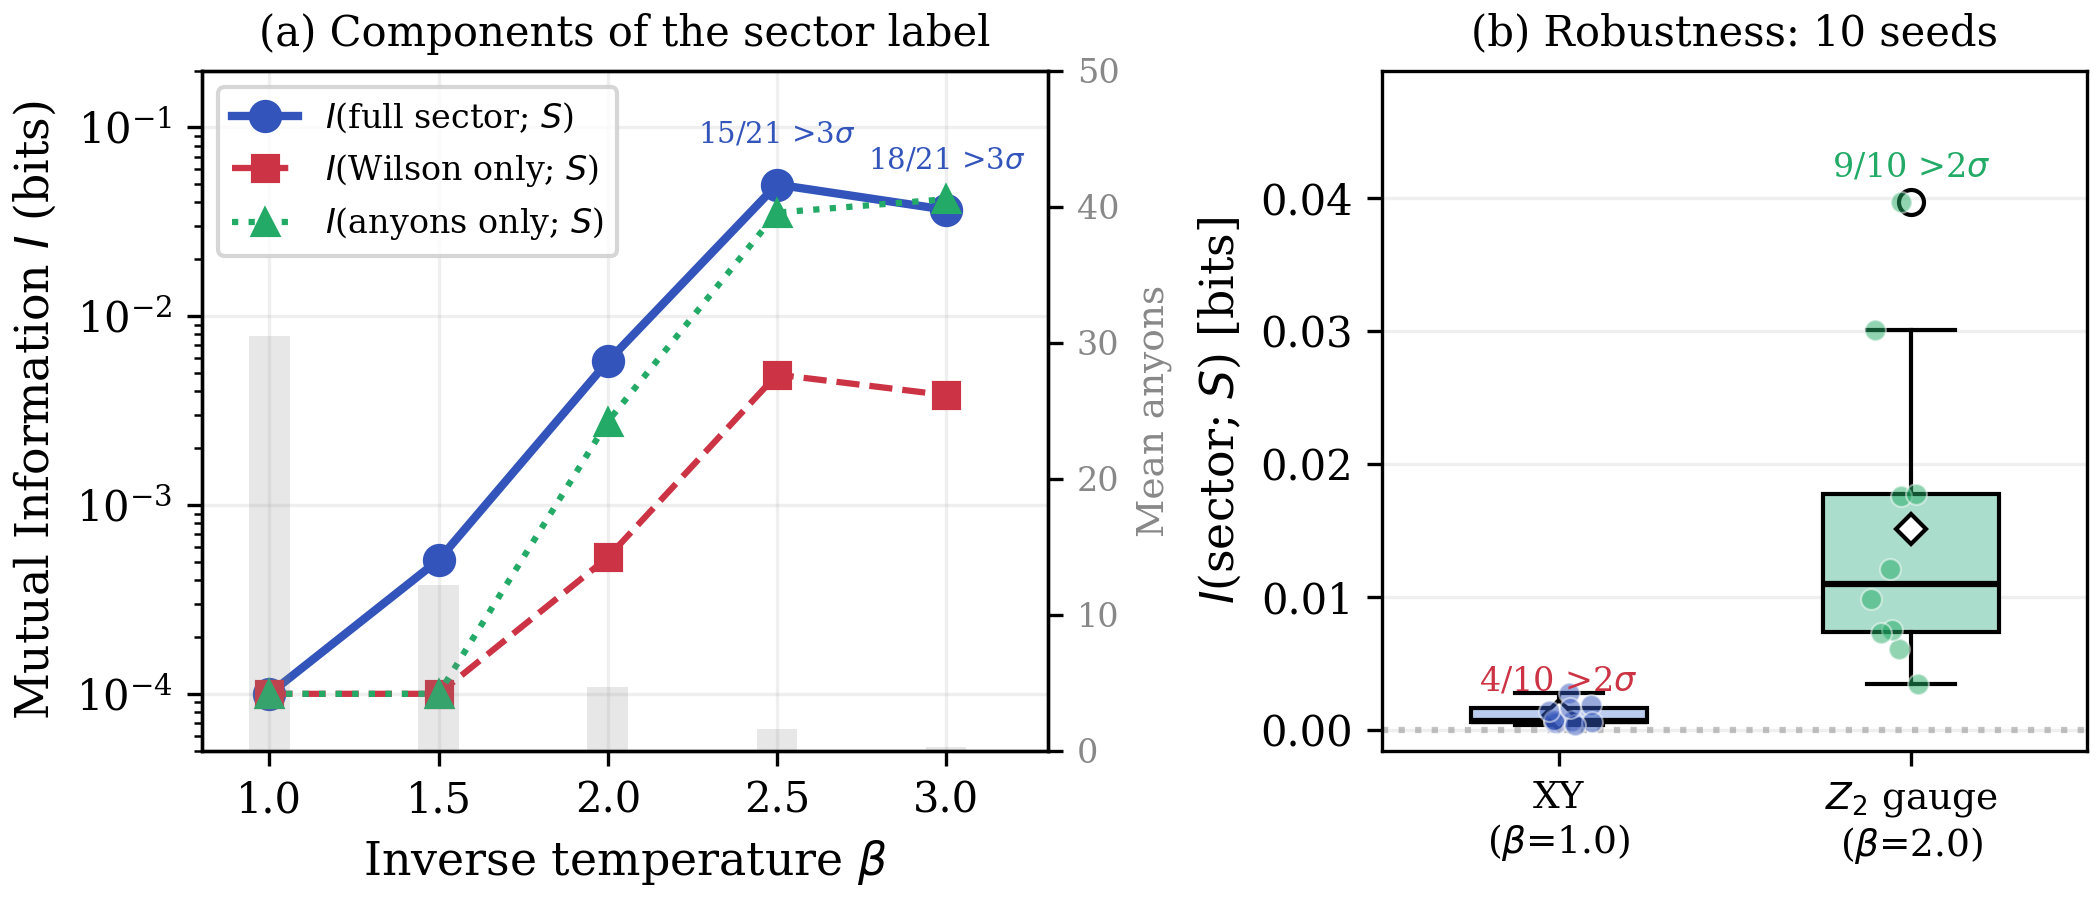
\includegraphics[width=\textwidth]{figures/fig1_crossover_seeds.png}
  \caption{(a)~Mutual information vs.\ inverse temperature for the components of the sector label (corrected engine, 21 seeds, circular-shift null subtracted; Table~\ref{tab:crossover}). Gray bars: mean anyon count. (b)~Seed variation: 10 independent runs per model (original analysis; for $\Ztwo$ the seeds of Table~\ref{tab:seeds}). Values in (a) are clipped at $10^{-4}$ for the logarithmic axis.}
  \label{fig:crossover}
\end{figure*}

\subsection{Finite-Size Scaling of $\MI$}
\label{sec:z2_scaling}

\paragraph{Motivation.}
The $\MI = 0.015 \pm 0.011$~bits (standard deviation across seeds) reported as the original analysis in the previous subsection is a
measurement at fixed lattice size $L=16$ and fixed temperature $\beta=2.0$.
A natural question, raised by gauge-theory generalities, is how this signal
scales with $L$: does it persist toward the thermodynamic limit, or is it a
finite-size effect of the $L=16$ system used for the original measurement? We
report here a dedicated scaling study at fixed $\beta=2.0$. The aim is not to
retract the $L=16$ value but to embed it in a scaling sequence.

\paragraph{Methods.}
We measure $\MI$ at $L \in \{8, 16, 32, 48, 64\}$, $\beta = 2.0$, with $10$
independent random-seed runs per $(L,\text{engine})$ cell. Two independent
Monte~Carlo engines are used, sharing the single-spin-flip Metropolis update
rule but differing in sweep order: (i)~the legacy engine
\texttt{z2\_sim\_v05.py} (same as for the original analysis of Table~\ref{tab:seeds})
sweeps the link variables in row-major order; (ii)~a newly written vectorized
engine \texttt{z2\_vec.py} updates the link variables in a checkerboard order.
The two engines are compared against the analytic single-plaquette expectation
$\langle B_p \rangle = \tanh(\beta)$ (Wegner duality limit, exact for the 2D
$\Ztwo$ gauge model at the level of single-plaquette averages). Statistical significance per cell is reported as $\sigma = (\bar I_\mathrm{real} - \bar I_\mathrm{shuffled}) / \sqrt{\mathrm{SEM}_\mathrm{real}^2 + \mathrm{SEM}_\mathrm{shuffled}^2}$, the difference of the seed means divided by their combined standard error across the 10 seeds, with $2000$ permutation shuffles per seed. Three model classes are
pre-registered for the $L$-dependence fit: a pure power law $M_2 :
a L^{b}$; a power law with nonzero asymptote $M_{2c} : a L^{b} + c$; and a
constant-asymptote exponential $M_\mathrm{exp} : a e^{-b L} + c$. Model selection
is by Bayesian information criterion (BIC), with $\Delta\mathrm{BIC} > 6$ used
as the threshold for decisive preference among the three.

\paragraph{Results --- per-cell measurements.}
Table~\ref{tab:z2_scaling} reports $I_\mathrm{mean} \pm \mathrm{SEM}$ over the
10 seeds per cell, together with the standardized significance against the
permutation null. The legacy-engine value at $L=16$, $I = 0.0149 \pm 0.0036$~bits,
reproduces the original-analysis mean of Table~\ref{tab:seeds}
($0.015 \pm 0.011$~bits, standard deviation across seeds) to within
$0.03\sigma$.

\begin{table}[b]
\caption{Mutual information $\MI$ vs.\ lattice size $L$ at fixed $\beta=2.0$, 10 seeds per cell: original analysis on the two superseded engines (legacy v05, vectorized vec; disclosure in the text). $\sigma$ is the difference of the seed means of $\MI$ and of its permutation surrogates (2000 shuffles per seed), divided by their combined standard error across seeds. The corrected engine's values are given in the text.}
\label{tab:z2_scaling}
\begin{ruledtabular}
\begin{tabular}{rcccc}
$L$ & v05: $I$ (bits) & $\sigma$ & vec: $I$ (bits) & $\sigma$ \\
\hline
 8 & $0.0372 \pm 0.0108$    & 3.5 & $0.0191 \pm 0.0029$     & 6.6 \\
16 & $0.0149 \pm 0.0036$    & 4.1 & $0.00694 \pm 0.00144$   & 5.1 \\
32 & $0.00235 \pm 0.00069$  & 2.5 & $0.000544 \pm 0.000628$ & 0.6 \\
48 & $0.000091 \pm 0.000315$ & 0.3 & $-3.5\!\times\!10^{-6} \pm 6.1\!\times\!10^{-5}$ & 0.2 \\
64 & $0.0000857 \pm 0.0000461$ & 0.6 & $2.9\!\times\!10^{-7} \pm 2.1\!\times\!10^{-5}$ & 0.5 \\
\end{tabular}
\end{ruledtabular}
\footnotetext{All cell-level values reproducible from
\texttt{data/stufe2\_analyse.json} (included in this release), which
\texttt{data/stufe2\_analyse.py} regenerates from the raw run
\texttt{data/stufe2\_results.json}; seeds 10--19 systematic. The $\sigma$
column is the field \texttt{sig\_minus\_scrambled} of that file.}
\end{table}

\paragraph{BIC model comparison.}
Three model classes are pre-registered for the $L$-dependence of the
sector-shuffle-corrected $\MI(L)$ at $\beta=2.0$ (the raw $\MI$ minus the mean
$\MI$ of sector-shuffled surrogates, i.e., the permutation-null-subtracted
signal reported per cell in \texttt{data/stufe2\_analyse.json}): a pure power law
$M_2 : a L^{b}$ (2 parameters); a power law with nonzero asymptote
$M_{2c} : a L^{b} + c$ (3 parameters); and a constant-asymptote exponential
$M_\mathrm{exp} : a e^{-b L} + c$ (3 parameters). Table~\ref{tab:z2_bic}
reports BIC and $\chi^2$ for each model and each engine.

\begin{table}[b]
\caption{Bayesian information criterion (BIC) for three pre-registered
$L$-scaling models of $\MI(L)$ at $\beta=2.0$, fitted to
Tab.~\ref{tab:z2_scaling}. $\chi^2$ is the unweighted sum of squared
residuals. $\Delta\mathrm{BIC}_\mathrm{best\,vs\,2nd}$ above $6$ is the
pre-registered threshold for decisive preference; $2$--$6$ counts as positive
evidence. Original analysis on the two superseded engines; no model comparison was computed for the corrected engine.}
\label{tab:z2_bic}
\begin{ruledtabular}
\begin{tabular}{lrrrr}
Model & v05: BIC & v05: $\chi^2$ & vec: BIC & vec: $\chi^2$ \\
\hline
$M_2$                            & 12.33         & 9.11         & 15.77         & 12.55 \\
$M_{2c}$                         &  8.26         & 3.44         & 12.86         &  8.03 \\
$M_\mathrm{exp}$ (best)          & \textbf{5.11} & \textbf{0.28} & \textbf{5.69} & \textbf{0.86} \\
\hline
$\Delta\mathrm{BIC}_\mathrm{best\,vs\,2nd}$ & \multicolumn{2}{c}{3.15} & \multicolumn{2}{c}{7.18} \\
\end{tabular}
\end{ruledtabular}
\footnotetext{Fit parameters and per-$L$ predictions reproducible from
\texttt{data/stufe2\_analyse.json}.}
\end{table}

\paragraph{Engine consensus.}
$M_\mathrm{exp}$ minimizes BIC in both engines (Fig.~\ref{fig:z2_scaling}). The strength of the preference
differs: in the vectorized engine
$\Delta\mathrm{BIC}_\mathrm{best\,vs\,2nd} = 7.18$, above the pre-registered
decisive threshold; in the legacy engine the gap is $3.15$, positive but
sub-decisive. Given the sub-decisive gap in the legacy engine, the
engine-consensus carries the model-selection conclusion, not either engine
alone --- $M_\mathrm{exp}$ is the \emph{preferred} model among the
pre-registered set, not a uniquely determined one. The fitted exponential rate
is consistent across engines: $b = 0.125 \pm 0.020$ (v05) and
$b = 0.140 \pm 0.024$ (vec), corresponding to a characteristic length scale of
$1/b \approx 7$--$8$ lattice spacings. The fitted asymptote $c$ is statistically
indistinguishable from zero in both engines:
$c = (0.62 \pm 8.8) \times 10^{-5}$ (v05) and
$c = (0.10 \pm 3.2) \times 10^{-5}$ (vec), each with
$|c|/\mathrm{SEM}(c) < 0.1$. Two qualitative conclusions follow that are
robust across both superseded engines: (i)~$\MI(L)$ decays faster than any power law
in the tested range, and (ii)~the asymptote is data-supported (not
extrapolated) to be indistinguishable from zero. The corrected engine (10 seeds per cell, circular-shift null) gives $0.0248$ $[0.0143, 0.0360]$~bits at $L = 8$ and $0.0051$ $[0.0026, 0.0074]$~bits at $L = 16$, and $95\%$ intervals that include zero from $L = 32$ on; conclusion~(ii) therefore holds on all three engines, while the model comparison behind conclusion~(i) rests on the superseded engines. The absolute $L=16$ value
is, however, \emph{not} engine-robust --- see disclosure below.

\paragraph{Superseded engines --- disclosure.}
The two engines do not agree on the absolute $\MI$ value at fixed $(L,\beta)$.
At $L=16$, $\beta=2.0$, the legacy engine reports $I = 0.0149 \pm 0.0036$~bits
while the vectorized engine reports $I = 0.00694 \pm 0.00144$~bits, a factor of
$\sim 2.15$. The two engines also differ in their reproduction of the analytic
single-plaquette expectation $\langle B_p \rangle = \tanh(\beta)$
(Wegner-duality limit, exact for the 2D~$\Ztwo$ gauge model at the level of
single-plaquette averages): at $\beta=2.0$ the legacy engine deviates by $+2.2\%$ toward colder configurations (original diagnostic), and the deposited validation shows that the vectorized update, too, misses the exact finite-torus value, by $+0.66\%$ at $L = 16$. The mechanism has since been isolated. The legacy engine visits the links in a fixed row-major order and accepts every energy-neutral flip deterministically; together these make its Markov chain reducible, so that time averages depend on the starting configuration. The vectorized engine shares the deterministic acceptance and is biased by it. The corrected engine accepts energy-neutral flips with probability $1/2$ and otherwise keeps the vectorized update. Against the exact plaquette average of the finite torus, of which $\tanh(\beta)$ is the unconstrained limit, it passes at all four validation points to within $1.2$ standard errors, while the same engine without this change misses by $4.3$ to $52.6$ standard errors. All $\Ztwo$ values in Sec.~\ref{sec:results} and in Tables~\ref{tab:crossover} and~\ref{tab:gauge_inv} are from the corrected engine. The plaquette diagnostic does not, by itself, \emph{select} among the
three scaling models above; model selection rests on the BIC comparison of
Tab.~\ref{tab:z2_bic}. The previously reported $I = 0.015 \pm 0.011$~bits (standard deviation across seeds) at $L=16$ (Sec.~\ref{sec:results}) remains a correct measurement of the legacy engine's output, and the corrected engine reproduces it as a raw value ($0.0150$~bits over 21 seeds; $0.0152 \pm 0.0012$~bits, standard error, on the scaling seeds). What does not carry over is the per-seed significance attached to it (Sec.~\ref{sec:results}). The vanishing asymptote of the consensus paragraph holds on all three engines.

\begin{figure*}[t]
  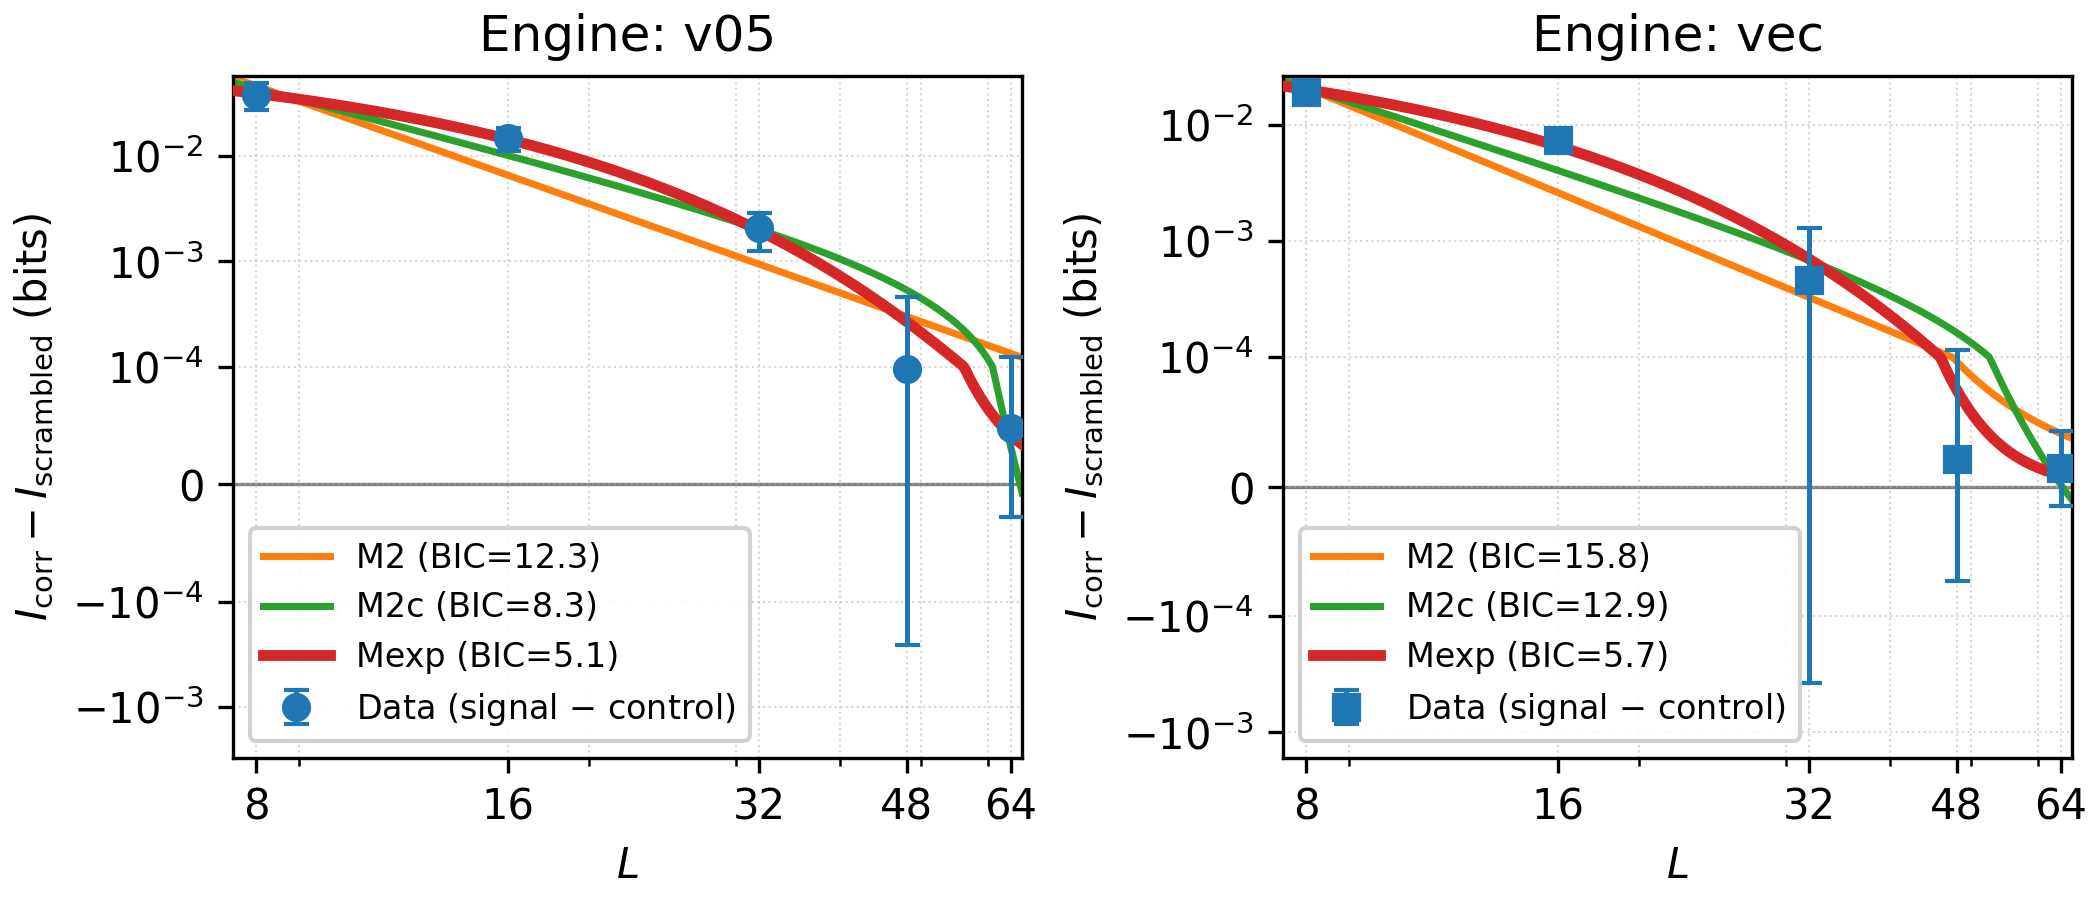
\includegraphics[width=\textwidth]{figures/fig4_z2_scaling.png}
  \caption{Finite-size scaling of $\MI$ in 2D $\Ztwo$ gauge theory at
  $\beta=2.0$. Per-cell measurements (Tab.~\ref{tab:z2_scaling}) with two
  Monte-Carlo engines (legacy v05 = circles, vectorized vec = squares) and
  the three pre-registered fit curves (Tab.~\ref{tab:z2_bic}): pure power
  $M_2$, power-with-asymptote $M_{2c}$, exponential $M_\mathrm{exp}$.
  $M_\mathrm{exp}$ is the BIC-preferred model in both engines (decisive in
  vec, sub-decisive in v05). The engine-consensus conclusion is qualitative:
  $\MI(L)$ decays faster than any power law in the tested range, with asymptote data-supported
  to be zero within the measurement precision. The absolute $L=16$ value is
  engine-specific (see disclosure in text). Original analysis on the two superseded engines; the corrected engine's per-cell values are given in the text.}
  \label{fig:z2_scaling}
\end{figure*}

\paragraph{Conclusion.}
The subsection has two robust takeaways and one scope-limiting statement.
\emph{Robust:} (i)~at fixed $\beta=2.0$, $\MI(L)$ decreases faster than any
power law in the tested range $L \in \{8,16,32,48,64\}$, with the
exponential form $M_\mathrm{exp}$ preferred under the pre-registered set in
both engines; (ii)~the asymptote is data-supported (not extrapolated) to be statistically indistinguishable from zero, also for the corrected engine. \emph{Engine-specific:} the
absolute $L=16$ value differs by a factor of $\sim 2$ between the two
engines and should be read as engine-specific (legacy: $0.0149$~bits, vectorized: $0.00694$~bits; the corrected engine gives $0.0152$~bits); the qualitative trend is unaffected by this
specificity. \emph{Scope.} The methodological question of how a
finite-size $\MI > 0$ at $L=16$ that decays toward zero at larger $L$
should be interpreted --- in particular, whether the observed signal admits
a non-finite-size physical reading --- is beyond the empirical scope of this
paper and is deferred to future theoretical work.

\subsection{XY Model: Exploratory}

In the XY model at $\beta = 1.0$, seed variation reveals that $I(|n|;\,S)$ is not
robust: only 4/10 runs exceed $2\sigma$ (2/10 ${>}3\sigma$). Mean:
$I = 0.001 \pm 0.001$~bits at $1.5 \pm 1.9\,\sigma$. The trend
$\uparrow|n| \to \downarrow S$ has correlation $r = +0.03 \pm 0.75$, consistent
with zero. We report this as exploratory. The signal may require larger lattices
or longer runs to establish in this noisier model.

Vortex-antivortex correlations show Coulomb-like attraction ($g(r{=}1) = -0.78$)
consistent with BKT physics~\cite{KT1973}, and the CHSH value anti-correlates
with defect count ($r = -0.90$), indicating that topological disorder degrades
CHSH correlations.

\subsection{Quantum Toric Code}

At $L = 2$ (8~qubits), $m$-anyon pairs yield $|S| = \sqrt{2}$ with the sign
flipping between sectors ($I = 0.350$~bits, $1595\sigma$). At $L = 3$
(18~qubits), all single-qubit and Wilson-loop correlations are exactly zero ---
verified across all 153 qubit pairs and all operator types
($\sigma^z$-$\sigma^z$, $\sigma^x$-$\sigma^x$, mixed).

The $L = 2$ result is a finite-size artifact: on a $2 \times 2$ torus,
measurement qubits simultaneously belong to the string, the plaquettes, and
noncontractible loops. At $L \geq 3$, the abelian nature of $\Ztwo$ anyons means
their entanglement is encoded globally and cannot be accessed by any operator that
is a product of Pauli matrices on a contractible subset of edges~\cite{Wen2002,Nayak2008}.

\subsection{Systematic Negative Results}

We tested three classical mechanisms for Bell violation:

\textbf{(i)~Measurement-rule modification:} Making $A(a, \lambda)$ depend on the
topological sector~$n$ via a phase shift
$A = \mathrm{sign}(\cos(a - \theta + n\alpha))$ \emph{decreases} $|S|$ --- the
coupling adds noise rather than correlation.

\textbf{(ii)~Statistical-independence violation:} Weighting configurations by
$\rho(n|a,b)$ allows $S$ to reach 2.000 exactly but never exceed it. Fine's theorem~\cite{Fine1982}
guarantees $|S| \leq 2$ for deterministic local functions $A(a, \lambda)$ and
$B(b, \lambda)$ only when the hidden-variable weighting $\rho(\lambda)$ is
\emph{setting-independent}; the present family $\rho(n|a,b)$ is explicitly
setting-dependent, so the theorem's hypothesis is not strictly satisfied here. Our
result is narrower and empirical: this particular sector-mediated weighting family
caps at $S=2.000$ in the numerics tested, not a general re-derivation of the Fine
bound for setting-dependent weightings.

\textbf{(iii)~Transport phase:} Including a gauge-field phase accumulated along
the path between detectors produces the correct angular form (correlation with
$-\cos\theta$ at $r = 0.993$) but only 17\% of the quantum-mechanical amplitude.
Thermal fluctuations wash out the phase coherence.

\begin{figure*}[t]
  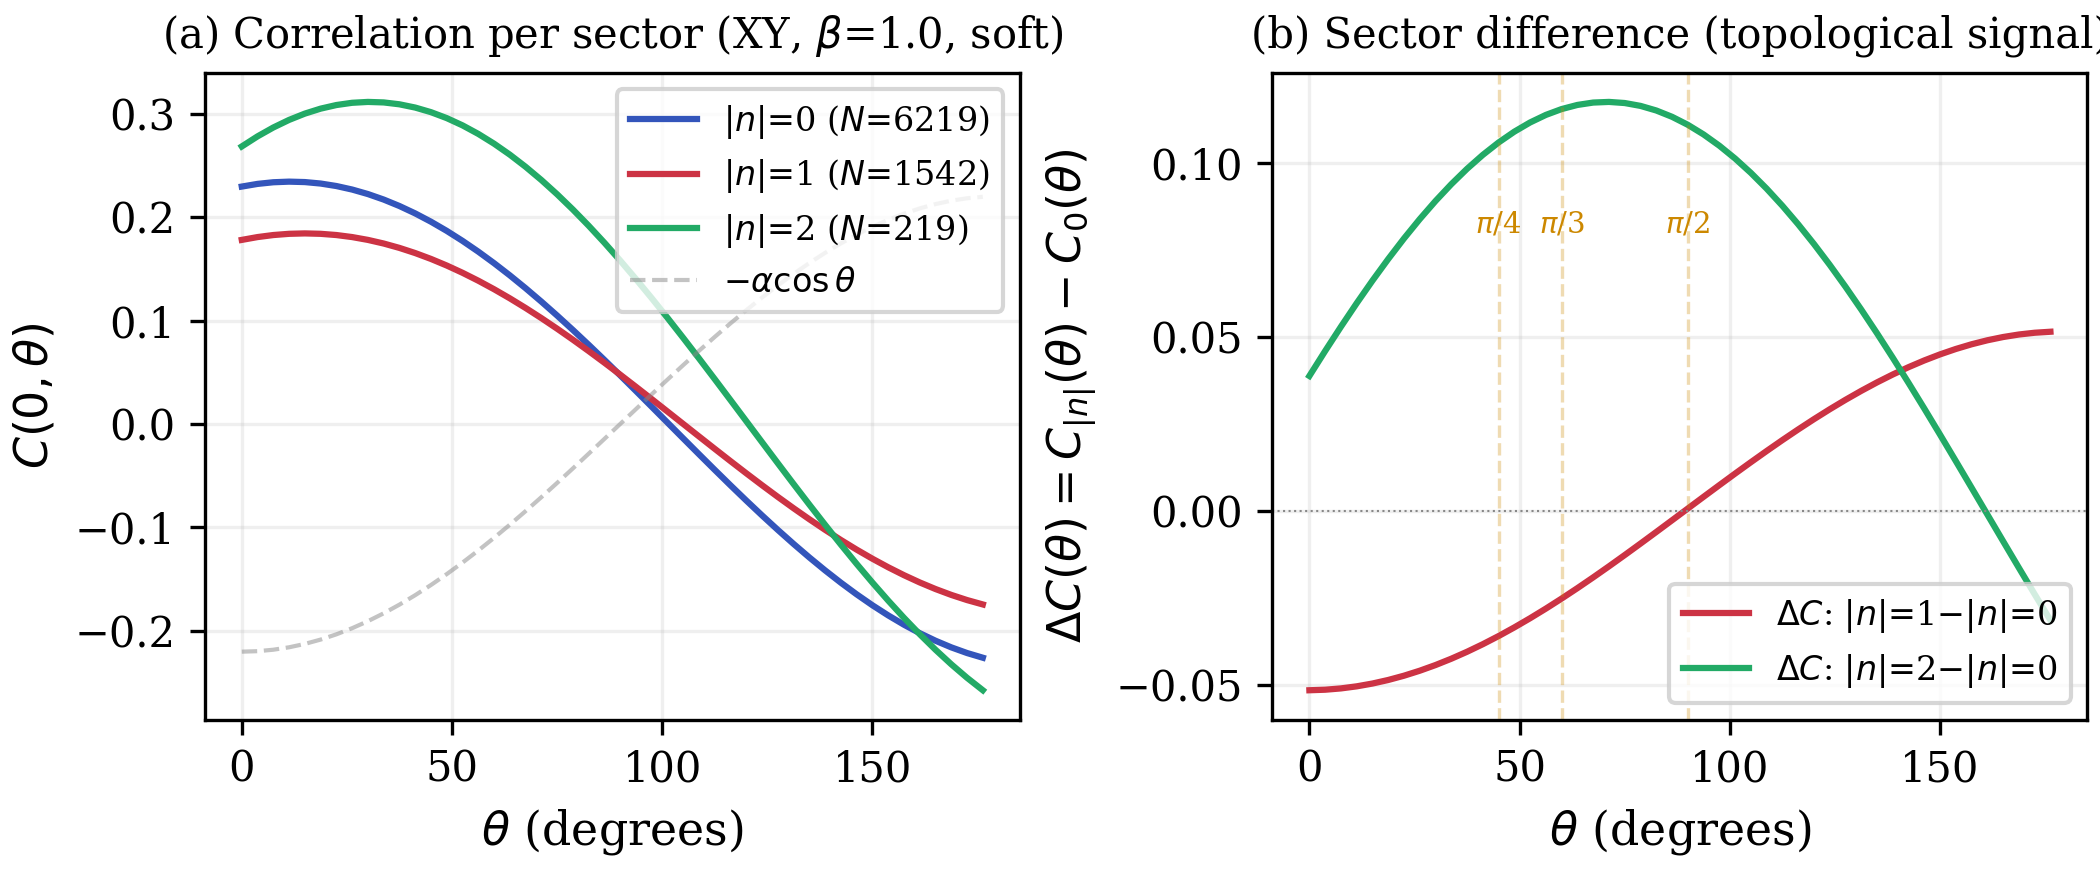
\includegraphics[width=\textwidth]{figures/fig2_sector_correlation.png}
  \caption{(a)~Correlation $C(0, \theta)$ per winding-number sector in the XY
  model (soft measurement). (b)~Sector difference
  $\Delta C = C_{|n|}(\theta) - C_0(\theta)$, isolating the topological signal.
  Dashed lines mark predicted resonance angles $\pi/n$.}
  \label{fig:sector_corr}
\end{figure*}

\subsection{Fourier Analysis}

The sector difference $\Delta C(\theta)$ (Fig.~\ref{fig:sector_corr}) shows the dominant Fourier mode is
$k = 1$ in all sectors, inconsistent with the prediction that the mode should
scale with winding number~$n$. A weak resonance enhancement at $\theta = \pi/n$
for $|n| \geq 2$ (amplitude ratio 1.20--1.38) is observed but not statistically
decisive. The even-harmonic structure in raw residuals ($a_2 \gg a_1$) is an
artifact of the $\mathrm{sign}(\cos)$ measurement discretization, eliminated by
using soft ($\cos$) measurements.

\subsection{Fibonacci Anyons: CHSH-Form Values}
\label{sec:fibonacci}

Fibonacci anyons have fusion rule $\tau \times \tau = 1 + \tau$ (golden ratio
quantum dimension) and no fermion parity superselection. Their braiding generates
a dense subset of $\mathrm{SU}(2)$ per logical qubit, making them universal
for quantum computation~\cite{Freedman2003}. We simulate two logical qubits
encoded in six Fibonacci anyons with the $d_{1b}$ circuit model, a two-qubit
circuit whose gates are constructed from the Fibonacci $F$-matrix
\begin{equation}
  F = \begin{pmatrix} \varphi^{-1} & \varphi^{-1/2} \\
  \varphi^{-1/2} & -\varphi^{-1} \end{pmatrix},
  \quad \varphi = \tfrac{1+\sqrt{5}}{2},
  \label{eq:fib_f_matrix}
\end{equation}
and $R$-matrix ($R_1 = e^{-4i\pi/5}$, $R_\tau = e^{3i\pi/5}$). One gate acts
on Alice's qubit alone, the other acts on Bob's qubit conditioned on Alice's;
the two gates do not satisfy the braid relations. We denote them AM and MB.
Braiding alone, with the two commuting braid generators of the same encoding,
does not exceed $|S| = 2$ (Ref.~\cite{Sayim2026fibonacci}).

Table~\ref{tab:fibonacci} shows the maximal CHSH value as a function of
sequence length. No enumerated sequence from $L=3$ to $L=12$ falls
below the classical CHSH bound: each either violates it ($|S|>2$) or
saturates it exactly ($|S|=2$ to within $10^{-10}$). The violating fraction at
$\delta = 0$ rises monotonically from $4/8$ at $L=3$ to $4077/4096$ at $L=12$. The
maximum $|S|$ over the 50-point $\delta$-grid rises monotonically from $2.199$
at $L=3$ to $|S|=2.811$ at $L=12$ ($99.4\%$ of the Tsirelson bound
$2\sqrt{2}$, $C=0.988$, at $\delta \approx 1.44\pi$); at $\delta = 0$, with
the standard Fibonacci data, the $L=12$ maximum is $|S| = 2.733$ ($96.6\%$, $C
= 0.932$).
These $|S|$ values are signatures of nonseparability on the nonfactorized
Fibonacci fusion space, not Bell violations in the
Einstein--Podolsky--Rosen bipartite sense.
The optimal length-12 sequence on the grid (at $\delta \approx 1.44\pi$) is
$(\text{AM}\cdot\text{MB})^6$, where AM acts on Alice's qubit alone and MB on
Bob's qubit conditioned on Alice's.
Both values are exact within the model at their $\delta$
--- $2.733$ with the standard data at $\delta=0$, $2.811$ with the deformed
data at $\delta\approx1.44\pi$ --- and were obtained by full enumeration
over all $2^L$ sequences combined
with the Horodecki bound $|S|_{\max} = 2\sqrt{1+C^2}$~\cite{Horodecki1995}, as
detailed in the companion paper Ref.~\cite{Sayim2026fibonacci}; see
\textit{Note on optimization} below for the v2.0 $\to$ v2.1 correction.


\begin{table}[b]
\caption{Fibonacci anyon CHSH-form values vs.\ sequence length
(values reproduced from Ref.~\cite{Sayim2026fibonacci} Tab.~I via full enumeration
over all $2^L$ sequences and the 50-point $\delta$-grid; the $|S|$, $C$, \%
Tsir., $\delta^*/\pi$, and sequence columns give the best sequence at a grid
point $\delta^*$ that maximizes $|S|$ (the mirror-image point
$6\pi/5-\delta^*$, mod $2\pi$, gives the same value),
and $\delta = 0$ carries the standard Fibonacci data, where
$L = 12$ gives $|S| = 2.733$; Horodecki bound
$|S|_{\max} = 2\sqrt{1+C^2}$~\cite{Horodecki1995} from the maximal
concurrence~$C$).  The last column counts how many of the $2^L$ sequences
violate at $\delta = 0$; the preceding columns report the single best sequence.
Sequence notation: $A = \text{AM}$ (gate on Alice's qubit), $B = \text{MB}$
(gate on Bob's qubit conditioned on Alice's).}
\label{tab:fibonacci}
\scriptsize
\begin{ruledtabular}
\begin{tabular}{rcccccc} $L$ & $|S|$ & $C$ & \% Tsir. & $\delta^*/\pi$ &
Sequence & Viol.\ ($\delta{=}0$) \\
\hline
 3 & 2.199 & 0.457 & 77.7 & 0.08 & ABB & 4/8 \\
 4 & 2.225 & 0.488 & 78.7 & 1.40 & ABAB & 11/16 \\
 5 & 2.348 & 0.615 & 83.0 & 1.44 & AABAB & 26/32 \\
 6 & 2.433 & 0.693 & 86.0 & 1.48 & AAABAB & 57/64 \\
 7 & 2.536 & 0.780 & 89.7 & 0.12 & ABBAABB & 120/128 \\
 8 & 2.540 & 0.783 & 89.8 & 1.36 & BABBABAB & 247/256 \\
 9 & 2.639 & 0.861 & 93.3 & 1.80 & ABBBBABAB & 502/512 \\
10 & 2.696 & 0.904 & 95.3 & 0.08 & ABBAABBAAB & 1013/1024 \\
11 & 2.784 & 0.968 & 98.4 & 1.44 & ABABBBBABAB & 2034/2048 \\
12 & \textbf{2.811} & \textbf{0.988} & \textbf{99.4} & \textbf{1.44} & \textbf{ABABABABABAB} & 4077/4096 \\\end{tabular}
\end{ruledtabular}
\footnotetext{The original v2.0 table reported lower $|S|$ values for
$L \leq 11$ from an X-Z-restricted angular optimizer; these have been replaced
in v2.1 by the Horodecki-bound full enumeration of Ref.~\cite{Sayim2026fibonacci}.  See
\textit{Note on optimization} below for the correction trail.}
\end{table}

The CHSH-form values depend strongly on $\delta$. When $\delta$ is varied
(modifying the relative phase between fusion channels),
the concurrence ranges from $0$ to $0.99$ over the
$\delta\in[0,2\pi)$ sweep ($N=200$ points). Throughout this Fibonacci sweep,
$\delta$ should be read as a representation-deformation parameter rather than
a physical anyon parameter: as verified numerically in the companion landscape
analysis [\cite{Sayim2026fibonacci}, Appendix~C], generic $\delta\neq0$ breaks
the Yang--Baxter/hexagon consistency of the braid representation, and only
$\delta=0$ realizes the standard Fibonacci modular tensor category. With \emph{fixed} measurement
settings (from a numerical search at the grid maximum $\delta\approx
1.44\pi$), $|S|$ ranges from near zero (when settings are misaligned with the
$\delta$-dependent optimal basis) to $2.72$, with $|S| > 2$ in $14\%$ of the
$200$ $\delta$ values.
When measurement settings are instead optimized at each $\delta$ via the full
Bloch-sphere parametrization (the same methodology used in
Table~\ref{tab:fibonacci}), the adapted-settings value is $|S|=2.811$
at $\delta\approx 1.44\pi$ and again at $\delta\approx 1.76\pi$: the sweep
takes the same value at both points, and the first of them is the one recorded
as the Table~\ref{tab:fibonacci} optimum at $L=12$. The two points are mirror
images about $\delta = 8\pi/5$: complex conjugation maps the generators at
$\delta$ to those at $6\pi/5 - \delta$ up to a global phase and leaves the
concurrence unchanged, so the whole sweep is mirror-symmetric (to within
$10^{-15}$ in the deposited data; $\delta = 6\pi/5$ reproduces the $\delta =
0$ value). On this finer 200-point sweep the maximum is $|S| = 2.816$, at
$\delta \approx 1.43\pi$ and $1.77\pi$, consistent with the grid value being a
lower bound.
With \emph{adapted}
settings via the Horodecki bound, $|S|$ never falls below $2.000$, and
$|S| > 2$ is achieved in $99.5\%$ of the $200$ $\delta$ values. Different
values of $\delta$ thus require different detector calibrations for the
maximum.

Unlike Ising anyons (Sec.~\ref{sec:ising_prediction}), Fibonacci anyons have no
fermion parity restriction on local measurements. The full Pauli algebra is
accessible in the fusion space, so measurements are not restricted by a parity
rule as they are for Ising anyons, whose protocol saturates at $S = 2.000$;
combined with the entangling gate MB, the $d_{1b}$ circuit model gives
CHSH-form values above 2, already at $\delta = 0$ ($|S| = 2.7334$). Among the
models compared in Fig.~\ref{fig:overview}, it is the only one that exceeds 2.
Braiding alone with the two generators of this encoding does not exceed 2
(Ref.~\cite{Sayim2026fibonacci}), so this excess is a property of the circuit
gates, not of braiding.

\paragraph{Note on optimization (added 2026-04-15, extended 2026-05-28).}
The length-12 grid maximum $|S| = 2.811$ ($\delta \approx 1.44\pi$) reported
here supersedes an earlier estimate
$|S| = 2.554$ obtained from the original angle-search optimizer (six random
seeds plus a $9^4$ grid). A subsequent full enumeration of winning sequences,
combined with the analytic Horodecki bound
$|S|_{\max} = 2\sqrt{1+C^2}$~\cite{Horodecki1995}, recovers $|S| = 2.811$ at
$C = 0.988$ for the grid-optimal length-12 sequence
$(\text{AM}\cdot\text{MB})^6$ at
$\delta\approx1.44\pi$ ($99.4\%$ of the Tsirelson bound).
The earlier value is therefore an optimization artifact, not a physical limit.
The same enumeration shows that the two encodings differ in the group they
generate: the two-generator $d_{1b}$ circuit model generates a six-dimensional
proper subgroup of $\mathrm{SU}(4)$ (entangling but not universal), while the
three-generator encoding is the standard $B_4$ braid representation on the
five-dimensional fusion space (dense on each intermediate-charge
sector~\cite{Bonesteel2005}); under standard four-dimensional
computational-subspace measurement both nevertheless reach comparable CHSH
values near the Tsirelson bound, differing primarily in the minimum word length
required ($L \approx 12$ vs.\ $L \approx 8$).
Protocol-dependent differences --- in particular the gap between native-$5$D
CHSH and the $4$D-projected value, and the associated leakage statistics ---
are documented in the companion paper
Ref.~\cite{Sayim2026fibonacci}.

\smallskip
\textit{v2.1 update (2026-05-28).}
The same Horodecki-bound full enumeration has been applied to lengths
$L = 3$--$11$ in v2.1, replacing the original X-Z-plane restricted angular
optimizer used in v2.0 (and earlier versions) for those rows of
Tab.~\ref{tab:fibonacci}.  The restricted optimizer reported systematically
lower values (mean deficit ${-}0.60$, maximum ${-}1.04$ at $L = 3$) and
suboptimal winning sequences, because complex-phase $R$-matrices in the
$d_{1b}$ circuit model require measurement operators rotated outside the X-Z
plane to saturate the Horodecki maximum.  With the corrected values, the trend
is monotonic in both $|S|$ and $C$ from $L=3$ to $L=12$; the earlier
"nonmonotonicity" interpretation in v2.0 was therefore an optimizer artifact
and has been removed.  See Ref.~\cite{Sayim2026fibonacci} Tab.~I for the underlying
enumeration.

\smallskip
\textit{Table~\ref{tab:fibonacci} update.}
Table~\ref{tab:fibonacci}, rows $L=6$ and $L=9$: the previously reported entries were the
maxima of an earlier $\delta$-sweep, not the maxima of the full
Horodecki-bound enumeration. They are replaced by the enumeration maxima
($L=6$: $|S|=2.433$, $C=0.693$, sequence AAABAB; $L=9$: $|S|=2.639$,
$C=0.861$, sequence ABBBBABAB). The remaining eight rows are unchanged.
The underlying enumeration is deposited with this record.

\section{Discussion}
\label{sec:discussion}

\subsection{Summary of Established Results}

We establish three main results at increasing levels of significance. First,
topological sectors and CHSH values are not statistically independent in the
$\Ztwo$ lattice gauge theory at $\beta = 2.0$ ($\MI = 0.0173$~bits on
gauge-invariant observables after subtracting the null level, $95\%$ interval
$[0.0159, 0.0187]$, $21$ of $21$
seeds ${>}3\sigma$ against a circular-shift null whose measured false-positive
level is $0.05$ of 21). The decomposition of Table~\ref{tab:crossover} shows
that the association is carried by the excitation-number component of the sector
label. The Wilson-loop component never dominates at any coupling examined, and
its own contribution is bounded at $1.2\times10^{-4}$~bits at $\beta = 1.0$,
where the sector label is maximally mixed ($1.9995$ of $2$~bits of entropy) and
effectively fully sampled ($3940$ of $4000$ measurements independent). The one
coupling at which its interval excludes zero, $\beta = 2.5$, is the one with the
poorest resolution among the couplings with a stated bound ($73$ of $4000$
independent), and the apparent
contribution grows as the resolution falls --- the signature of a residual
estimator bias rather than of physics. The origin of this mutual information is
therefore not topological. Second, this mutual-information signal is a
finite-size effect that decays toward zero with system size
(Sec.~\ref{sec:z2_scaling}). Third, and most significantly,
the two-generator $d_{1b}$ circuit model of Fibonacci anyons produces
CHSH-form values above 2: $|S| = 2.7334$ ($96.64\%$ of the Tsirelson bound) at
$\delta = 0$, the point that realizes the standard Fibonacci modular tensor
category, and $|S| = 2.8114$ ($99.40\%$) at the maximum of the 50-point
$\delta$-grid, $\delta \approx 1.44\pi$, both at sequence length $L = 12$; as
a grid maximum, $2.8114$ is a lower bound on the maximum over $\delta$. The
values depend strongly on $\delta$: with fixed detector settings, $|S|$ varies
from near zero to $2.72$ across $\delta \in [0, 2\pi)$.

The Fibonacci result contrasts with a hierarchy of negative results: $\Ztwo$ classical
models cannot violate Bell (Fine's theorem), abelian quantum anyons are locally
invisible ($L \geq 3$ toric code), and Ising anyons saturate at $S = 2.000$
(fermion parity). Fibonacci anyons have no parity restriction, and the
$d_{1b}$ circuit model built from their $F$- and $R$-matrices, with an
entangling gate, is the only model among those compared here that achieves
CHSH-form values above 2.

\smallskip
\noindent The models tested in this work, with the CHSH value reported for
each. Values are those of Tables~\ref{tab:fibonacci},~\ref{tab:history}
and~\ref{tab:negative}; the null results are listed because they carry the
statement that the $d_{1b}$ circuit model is the only one among those listed
here to exceed 2.
\smallskip
\begin{ruledtabular}
\footnotesize
\begin{tabular}{l l c}
Model & Setting & $|S|$ \\
\hline
XY $16{\times}16$ ($\beta{=}1.0$) & classical, $16{\times}16$ torus & 0.55 \\
XY + meas.\ coupling & classical, $16{\times}16$ torus & 0.80 \\
XY + $\rho(n|a,b)$ weighting & classical, $16{\times}16$ torus & 2.000 \\
XY + transport phase & classical, $16{\times}16$ torus & 0.44 \\
$\Ztwo$ gauge ($\beta{=}2.0$) & classical, $16{\times}16$ torus & 0.13 \\
$\Ztwo$ gauge ($\beta{=}3.0$) & classical, $16{\times}16$ torus & 1.34 \\
Quantum TC $L{=}2$ & exact diag., 8 qubits & 1.41 \\
Quantum TC $L{=}3$ & exact diag., 18 qubits & 0.00 \\
Perturbed TC ($h$-scan) & exact diag., 8 qubits & 0.00 \\
Ising anyons (Majorana) & Majorana rep. & 2.000 \\
\textbf{Fibonacci anyons} ($L{=}12$) & circuit, 4-D, $\delta{=}0$ & \textbf{2.733} \\
Fibonacci, deformed ($L{=}12$) & circuit, 4-D, $\delta{\approx}1.44\pi$ & 2.811 \\
\end{tabular}
\end{ruledtabular}

\subsection{Limitations}

All results reported here are numerical simulations within idealized TQFT
models, not laboratory experiments.
The Fibonacci CHSH violation is computed in the ideal TQFT fusion space --- a
unitary, zero-temperature, zero-decoherence model. In a physical realization
(e.g., $\nu = 12/5$ fractional quantum Hall state), thermal excitations,
finite system size, and quasiparticle tunneling would reduce $|S|$ below the
ideal value. In addition, the entangling gate of the circuit model is not a
braid (Ref.~\cite{Sayim2026fibonacci}), so a physical realization would have
to implement it by other means.
The $\Ztwo$ results are robust --- the corrected value is unchanged under a
tenfold longer run ($+0.0173$ against $+0.0179$~bits), while its significance
grows from $10.5$ to $74.8\sigma$, as a real effect does and an estimator bias
does not --- but small: $I \sim 0.01$--$0.04$~bits. The XY model result is not robust across seeds. The elevated mutual
information at $\beta = 2.5$ is carried by the excitation-number component of
the label, not by a nontrivial topological mechanism; the earlier reading of
that regime as a near-frozen anyon sector rested on the superseded engine.

\subsection{Implications for Topological Interpretations}

The Fibonacci result shows that, within the idealized TQFT model, the $d_{1b}$
circuit model with the standard Fibonacci $F$ and $R$ data ($\delta = 0$)
produces CHSH-form values above 2 with measurements on the two logical qubits
($|S| = 2.7334$). The sweep over $\delta$ is a deformation of the
representation, not a set of topological sectors, so it does not by itself
show a sector-dependent modulation; for Ising anyons, where the sector phase
is physical, the next subsection gives the analytic form of that dependence.

\subsection{Prediction: Sector-Dependent CHSH Correlations for Ising Anyons}
\label{sec:ising_prediction}

For Ising anyons we present an analytical argument that non-Abelian
topological order produces sector-dependent CHSH correlations. The Ising
braiding $R$-matrix has
two eigenvalues corresponding to the two fusion channels~\cite{Nayak2008,Kitaev2006}:
\begin{equation}
  R_1 = e^{-i\pi/8}, \qquad R_\psi = e^{3i\pi/8}.
  \label{eq:ising_r}
\end{equation}
On a torus, the topological sector modifies the relative phase between these
channels. In sector~$\delta$, the $R$-matrix becomes
$R_1 = e^{-i\pi/8}$, $R_\psi = e^{i(3\pi/8 + \delta)}$, where $\delta$ depends
on the anyon type threading the noncontractible loop~\cite{Kitaev2003,Kitaev2006}.
Here $\delta$ is a physical sector phase fixed by the threading anyon --- a
discrete, topologically determined label --- rather than a freely tunable
deformation parameter.
Braiding two pairs of Ising anyons produces the entangled fusion state:
\begin{equation}
  \ket{\psi(\delta)} = \cos\alpha\,\ket{00} + e^{i\delta}\sin\alpha\,\ket{11},
  \label{eq:ising_state}
\end{equation}
where $\alpha$ is determined by the braiding sequence and $\ket{0}$, $\ket{1}$
label the fusion channels (vacuum and fermion respectively). For maximal braiding
($\alpha = \pi/4$), the concurrence is 1 for all~$\delta$ --- the entanglement is
sector-independent. However, the CHSH value with \emph{fixed} measurement settings
is strongly sector-dependent:
\begin{equation}
  S(\delta) = 2\sqrt{2}\,\cos^2(\delta/2)
  \qquad\text{(settings optimized at $\delta{=}0$)}.
  \label{eq:s_delta}
\end{equation}

We verify this numerically: with settings optimized for the vacuum sector
($\delta = 0$), $S$ ranges from $2\sqrt{2} \approx 2.83$ (maximal CHSH violation)
at $\delta = 0$ to $S = \sqrt{2} \approx 1.41$ at $\delta = \pi/2$, and $S = 0$
at $\delta = \pi$, following the $\cos^2(\delta/2)$ law.
Eq.~(\ref{eq:s_delta}) is evaluated here as a continuous function of $\delta$;
values between the discrete sector values do not correspond to a physical
sector. Critically:

(i)~\textbf{CHSH violation is preserved in all sectors} if measurement settings
are adapted --- $\max|S| = 2\sqrt{2}$ for all~$\delta$. The topology does not
create or destroy entanglement.

(ii)~\textbf{With fixed settings, $S$ depends on the sector} --- producing
$\MI > 0$, the quantity measured for $\Ztwo$ in Sec.~\ref{sec:results}, here
with CHSH values above 2.

(iii)~\textbf{The sector rotates the optimal measurement basis} in the fusion
space. Different sectors require different detector calibrations to see maximum
violation. An observer who does not know the sector sees reduced~$S$ on average.

This constitutes a concrete analytical prediction, subject to the parity caveat
below: in any experiment that
creates and braids Ising anyons on a surface with nontrivial topology, the
observed CHSH value must depend on the topological sector. The functional form ---
$\cos$-modulation with period determined by the anyon type threading the handle
--- is parameter-free.

\textbf{Caveat:} Numerical verification via a Majorana fermion representation
shows that the braid-then-fuse measurement protocol saturates at $S = 2.000$
exactly for Ising anyons, due to the fermion parity superselection rule:
Pauli-$X$ operators project to zero in the even-parity sector, restricting local
measurements to the $Z$-basis. This limits Ising anyons to the classical bound when only
topologically protected stabilizer operations---gates and measurements
together---are available~\cite{HowardVala2012}. The prediction
$S(\delta) = 2\sqrt{2}\cos^2(\delta/2)$ applies when measurements in the full
fusion-space basis are available. Fibonacci anyons have no parity restriction,
but the $\delta$ sweep of Sec.~\ref{sec:fibonacci} is a deformation, not a
sector phase; the corresponding prediction for them is not derived here.
A companion paper~\cite{Sayim2026cbell}
constructs this noncommuting CHSH operator algebra locally in the Kitaev
honeycomb model; as noted above, a genuine violation with topologically
protected Ising operations requires nonstabilizer (magic) resources.

\subsection{Related Work and Prior Art}
\label{sec:related_work}

The CHSH-violation construction presented here for Fibonacci anyons sits in
a broader landscape of topological and nonstandard Bell tests. Earlier
qualitative Bell-test constructions for non-Abelian anyons were proposed by
Brennen, Iblisdir, Pachos, and Slingerland~\cite{Brennen2009} for Fibonacci
and Ising anyons; Chang, Chu, and Ma~\cite{ChangChuMa2017} studied Bell's
inequality in topologically ordered qubit models (Wen-plaquette). On Majorana
platforms, Drummond, Kovalev, Hou, Shtengel, and Pryadko~\cite{Drummond2014}
gave an explicit CHSH protocol for Majorana wires, and Romito and
Gefen~\cite{RomitoGefen2017} demonstrated nonlocal entanglement with six
Majorana zero modes reaching the Tsirelson bound. Single-particle Bell-like
inequality violations in neutron interferometry were reported by
Hasegawa, Loidl, Badurek, Baron, and
Rauch~\cite{Hasegawa2003}; the contextuality-based program of
Liu, Hu, Chen, Huang, Han, Li, Guo, and
Cabello~\cite{Liu2016Cabello} provides a complementary view on the relation
between nonlocality and contextuality. The present paper differs from these
works in scope: we report the mutual-information structure $I(T;S)$ between
topological sectors and CHSH values across a hierarchy of lattice and anyonic
models, including the finite-size scaling reported in
Sec.~\ref{sec:z2_scaling}, rather than a single Bell-test protocol on a fixed
topological platform.

Independently, Xu, Ye, and You~\cite{Xu2025} have
studied CHSH correlations on Fibonacci anyonic states using a three-copy
fusion-sector observables construction (their Eq.~(23)), reporting
$|S| \approx 2.633$ on $|\tau,\tau;1\rangle^{\otimes 3}$. Their setup differs
from ours in both the ambient fusion space and the observable choice; a
detailed setup-by-setup comparison appears in the companion
paper~\cite{Sayim2026fibonacci}.

Recent methodological work on braid-circuit verification by
Amaral~\cite{Amaral2025} and on minimal-depth Levin--Wen circuits by
Bseiso \emph{et al.}~\cite{Bseiso2024} provides additional methodological
context for the F-symbol conventions and Yang--Baxter checks used here. A
companion Leggett--Garg-inequality analysis using the same Fibonacci $F$- and
$R$-matrices, with $K_3$ values reaching $99.998\%$ of the L\"uders bound
$3/2$, is reported separately in Ref.~\cite{Sayim2026LGI}.

\subsection{Relation to Companion Work and Open Questions}

Two of the directions previously listed here are addressed elsewhere. The
complete enumeration of CHSH-form values over all words up to length $L=12$ in
the two-generator encoding is reported in the companion paper
Ref.~\cite{Sayim2026fibonacci}; that paper makes no claim about the
convergence of $|S|$ toward the Tsirelson bound for longer words. The
temporal-correlation counterpart, using the same Fibonacci $F$- and
$R$-matrices and Leggett--Garg-style protocols, is reported in
Ref.~\cite{Sayim2026LGI}. The finite-size scaling of
the $\Ztwo$ sector--CHSH mutual information is settled within the present paper
(Sec.~\ref{sec:z2_scaling}), where it is shown to decay toward zero with system
size. Two questions remain genuinely open. Whether a microscopic Hamiltonian
realization --- for example the Kitaev honeycomb model in its non-Abelian
phase~\cite{Kitaev2006} --- reproduces the sector dependence predicted for
Ising anyons in Sec.~\ref{sec:ising_prediction} is not established here. And
whether a physical sector phase produces a comparable dependence in other
non-Abelian anyon models, including Fibonacci anyons and $\mathrm{SU}(2)_k$
theories at level $k \geq 3$, is likewise not addressed by the present
construction.

\begin{figure*}[t]
  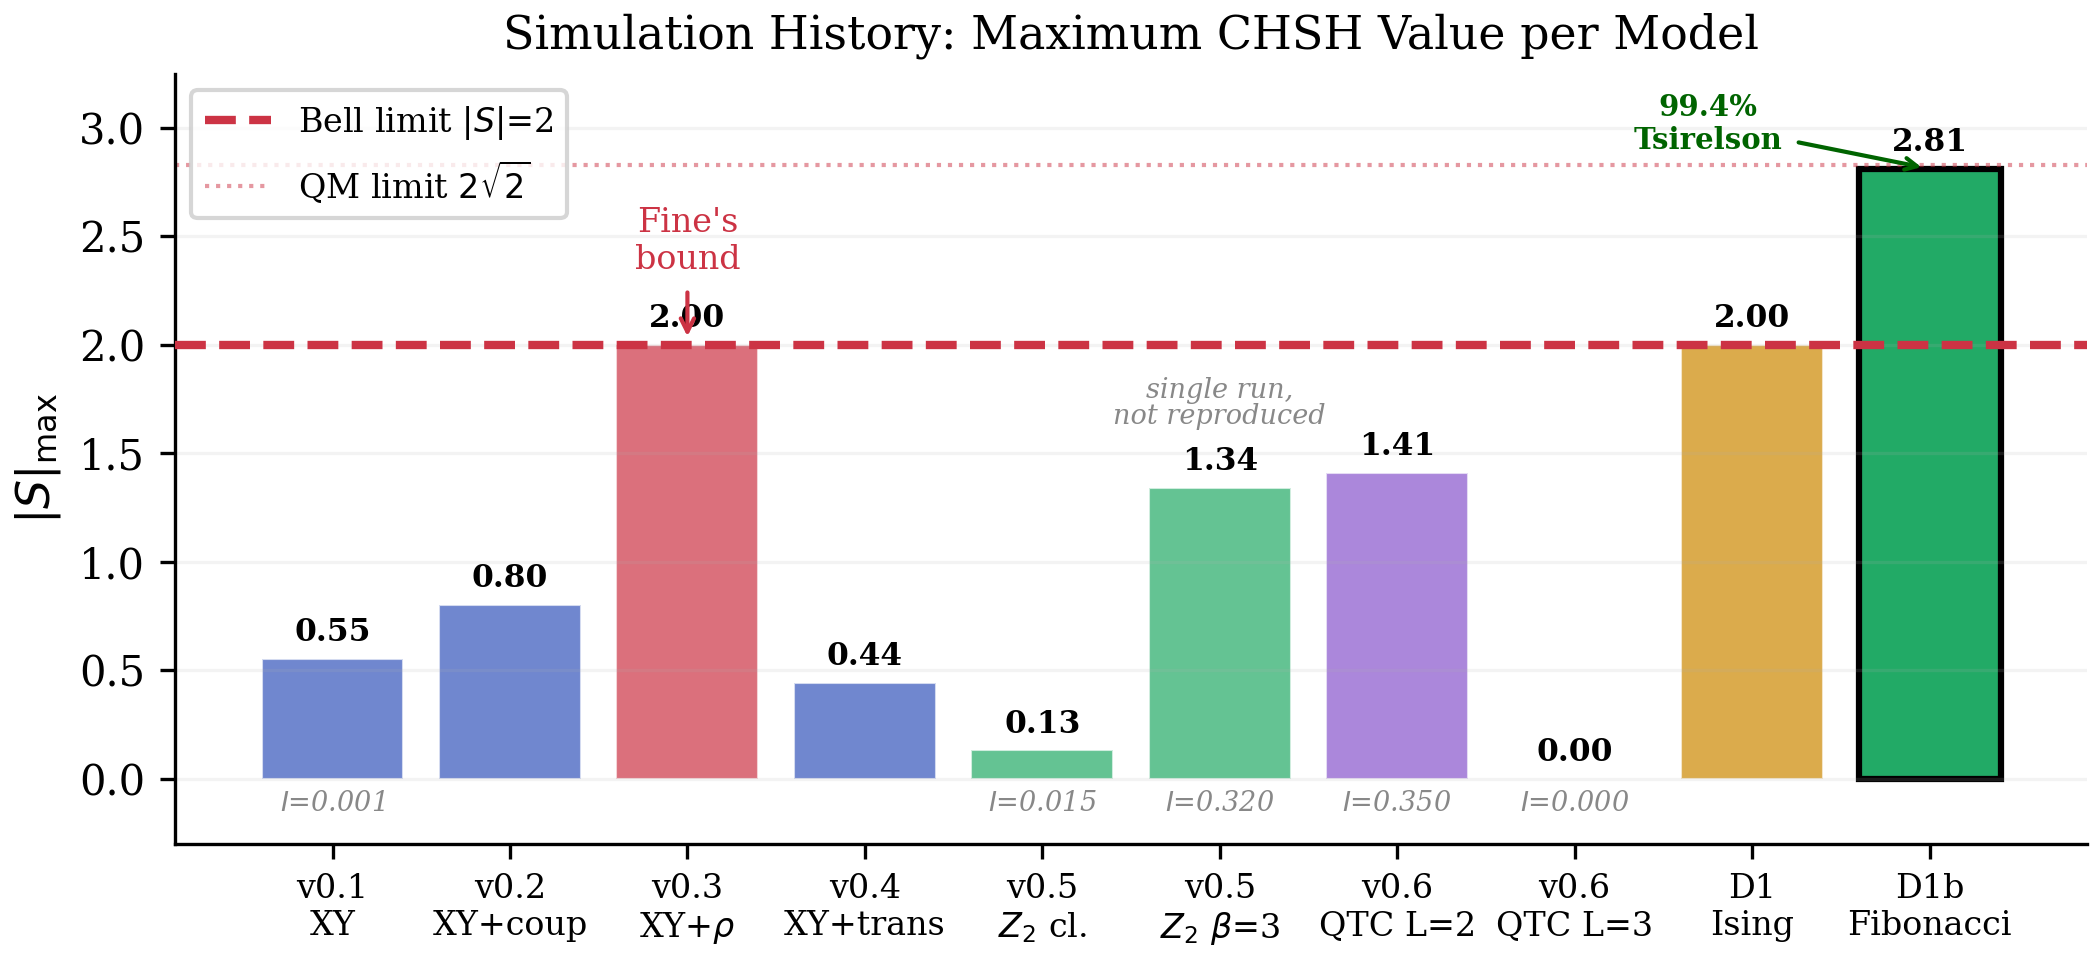
\includegraphics[width=\textwidth]{figures/fig3_overview.png}
  \caption{Maximum CHSH value across all simulation models. The classical limit
  $|S| = 2$ (dashed red) is never exceeded in abelian models. The Fibonacci
  bar ($L=12$) shows $|S| = 2.811$ ($99.4\%$ of the Tsirelson bound
  $2\sqrt{2}$; corrected value, see Note on optimization,
  Sec.~\ref{sec:fibonacci}), the maximum on the 50-point $\delta$-grid of the
  deformed representation ($\delta\approx1.44\pi$) and a lower bound on the
  maximum over $\delta$; at $\delta = 0$, the only point that realizes the
  standard Fibonacci modular tensor category, $|S| = 2.7334$.}
  \label{fig:overview}
\end{figure*}

\section{Conclusion}
\label{sec:conclusion}

We have presented a systematic numerical investigation showing that the
$d_{1b}$ circuit model with the standard Fibonacci data ($\delta = 0$)
produces CHSH-form values above 2 on the fusion space. The progression from
classical $\Ztwo$ gauge theory (a small, nontopological association: $\MI = 0.0173$~bits on gauge-invariant observables, carried by the excitation number) through
abelian quantum anyons (locally invisible at $L \geq 3$) to the $d_{1b}$
circuit model built from the Fibonacci $F$- and $R$-matrices ($|S| = 2.7334$
at $\delta = 0$) shows that, among the models compared in
Fig.~\ref{fig:overview}, only this circuit model exceeds $|S| = 2$; braiding
alone with the two generators of its encoding does not
(Ref.~\cite{Sayim2026fibonacci}).

Over the Fibonacci deformation sweep the CHSH-form values depend strongly on
$\delta$ (from near zero to $2.72$ with fixed settings; above 2 at $99.5\%$ of
the $\delta$ values with adapted settings), and the concurrence varies from
$0$ to $0.99$ (Sec.~\ref{sec:fibonacci}). For Ising anyons, where the sector
phase is physical, the analytic argument of Sec.~\ref{sec:ising_prediction}
predicts that the sector rotates the optimal measurement basis without
changing the entanglement, subject to the parity caveat stated there. The $\Ztwo$
mutual information is a finite-size, non-topological association, the Ising
analysis identifies the fermion parity obstruction, and the Fibonacci result
indicates that this obstruction is not universal. Together, they constitute a
systematic investigation of CHSH correlations across abelian and non-Abelian
models, with $I(\text{topology};\,\text{CHSH})$ measured in the lattice and
toric-code models.

\section*{Notation}
\noindent Symbols used in this paper.
\begin{ruledtabular}
\begin{tabular}{l p{0.72\columnwidth}}
Symbol & Meaning \\
\hline
$L$ & linear lattice size ($L\times L$ torus) or, for the anyon models, sequence length \\
$\beta$ & inverse temperature of the lattice model \\
$\langle B_p\rangle$ & single-plaquette expectation value \\
$\MI$ & mutual information between the topological sector label $T$ and the CHSH value $S$ \\
$|S|$ & magnitude of the CHSH functional \\
$C$ & concurrence of the two-qubit state \\
$\theta$ & measurement angle, $M(\theta)=\cos\theta\,\sigma^z+\sin\theta\,\sigma^x$ (lattice models) \\
$\text{AM},\text{MB}$ & the two circuit gates: AM acts on Alice's qubit alone, MB on Bob's qubit conditioned on Alice's \\
$\delta$ (Ising) & physical sector phase fixed by the anyon threading the noncontractible loop, $R_\psi=e^{i(3\pi/8+\delta)}$ \\
$\delta$ (Fibonacci) & representation-deformation parameter varied in the deformation sweep of Sec.~\ref{sec:fibonacci}; only $\delta = 0$ realizes the standard Fibonacci modular tensor category \\
\end{tabular}
\end{ruledtabular}

\section*{Data and Code Availability}
The seed statistics of Tables~\ref{tab:crossover} and~\ref{tab:gauge_inv} (means, intervals and counts) are those of the corrected engine's per-seed values deposited in \texttt{data/null\_calibration\_results\_vecrep\_v2.json}. The deterministic analysis scripts and JSON output files deposited with this record reproduce the finite-size
scaling of Tables~\ref{tab:z2_scaling} and~\ref{tab:z2_bic} (raw run in
\texttt{data/stufe2\_results.json}, aggregated by
\texttt{data/stufe2\_analyse.py} into the per-cell data and model comparison
of \texttt{data/stufe2\_analyse.json}), the frozen-regime characterization, and
Figs.~\ref{fig:crossover}(a) and~\ref{fig:z2_scaling}; the systematic seed sets
are $\{42, 10\text{--}29\}$ for the decomposition and both rows of Table~\ref{tab:gauge_inv}, and $10\text{--}19$ for the scaling cells. The
per-seed entries of Table~\ref{tab:seeds} are from the original analysis and
have no deposited generating script; its $L = 16$ mean is independently
reproduced by the deposited scaling run (Table~\ref{tab:z2_scaling}, v05
column, to within $0.03\sigma$). The original-analysis values in the footnote of Table~\ref{tab:gauge_inv} are reproduced, for the gauge-invariant route, by the deposited script \texttt{data/gauge\_inv\_plaquette\_strip\_recompute.py}; the independent re-implementation \texttt{data/gauge\_inv\_independent\_route.py} reproduces the count of 21 of 21 seeds above $3\sigma$. The gauge-fixed original values have no deposited generating script. The Fibonacci values of
Table~\ref{tab:fibonacci} are reproduced by the deposited enumeration
\texttt{data/fibonacci\_enumeration.py} and its output
\texttt{data/fibonacci\_enumeration\_results.json}, which cover all ten
lengths $L = 3$--$12$ and import the gate definitions read-only from the
companion record Ref.~\cite{Sayim2026fibonacci} (concept DOI
\href{https://doi.org/10.5281/zenodo.19601352}{10.5281/zenodo.19601352});
the $\delta$ sweep of one selected sequence per length for
$L = 3, 6, 8, 10, 12$ is held in that record's
\texttt{s\_delta\_sweeps.json}, which is deposited there and is not part of
the present package. The $\delta$ sweep behind the fixed- and
adapted-settings figures of Sec.~\ref{sec:fibonacci} --- $14\%$ and $99.5\%$ of
the $200$ sampled values, and the range up to $2.72$ --- is held in
\texttt{data/sector\_range\_fixed\_settings.json}, first deposited with
version~2.0 of this record
(\href{https://doi.org/10.5281/zenodo.19656928}{10.5281/zenodo.19656928}) and
included here. Its Horodecki column is reproducible from the deposited
concurrence column through $|S|_{\max} = 2\sqrt{1+C^2}$; the fixed-settings
angles come from a numerical search whose generating script is not deposited,
so those entries record what the deposited run yielded rather than what the
method yields on a re-run. The Ising
saturation $S = 2.000$ follows analytically from the fermion parity
superselection rule and is not a numerical result. The remaining entries of
Table~\ref{tab:history} and the corresponding bars of Fig.~\ref{fig:overview}
record earlier model iterations and are kept as history. All files are
archived on Zenodo under the concept DOI
\href{https://doi.org/10.5281/zenodo.19600752}{10.5281/zenodo.19600752} (which
always resolves to the latest version). Paper, figures, and data are released
under the Creative Commons Attribution 4.0 International (CC~BY~4.0) license;
the deposited source code is released under the Apache License 2.0 (see
\texttt{LICENSE} and \texttt{LICENSE-CODE}).

\section*{Use of AI tools}

In the research, processing, and writing of this paper and its results I worked together with generative AI tools, in practice a system of multiple coordinated AI instances that I set up and orchestrate (large language models, mainly Claude, by Anthropic, inside Claude Code). At their current context sizes I found it far more effective to work with several specialized instances, each with its own role and its own harness of rules and parameters that I designed and refined through feedback, than to load a single instance with all of the material; for my workflow that would have been inefficient, though this depends on the individual implementation. I lead this collaboration: I choose the research directions, set the goals, and make the final decisions in open exchange with the AI, learning actively as the work proceeds. The AI carries out the drafting, including the mathematical and technical parts, the numerical computation, and the literature search, under my direction. The AI works autonomously only task by task, within the structure I develop through feedback: it completes a task, and at open questions that need me it stops until the point is settled before the next step. Along the way I witness and take many of the decisions that shape the path, and it is common for me to spot things that need improvement. The work spans many separate runs, and a single simulation or build task alone can take up to an hour, so it could not happen all together in one autonomous run; and had I let the AI do all of it together alone, even if it is possible, it would no longer be my work but the AI's.

I run multiple verifications at the different stages of the work and one before release, including cross-checks with an unrelated AI model from a different company, and all references are checked against the original sources. In the end what matters are human eyes, a principle that is itself written into the parameters of my system: I reach out to experts after publishing for review and feedback, so I learn what is solid and what must be corrected or falsified. My scripts for reproduction and review are released with this record. These tools are not authors; I am the author, and I take full responsibility for all scientific content and decisions leading to these results and their publication.

\section*{Acknowledgments}
This research received no specific grant from any funding agency in the public,
commercial, or not-for-profit sectors. The author declares no competing
interests.

\clearpage
\onecolumngrid

\appendix
\section{Simulation Parameters and Negative Results}

All classical simulations use $L = 16$ with Metropolis MC (single-site for XY,
single-edge for $\Ztwo$). The legacy engine and the validation scripts thermalize for 2000~sweeps and take 4000~measurements per run (the frozen-regime characterization: 40\,000 measurements); an exploratory $\beta$ scan of the legacy engine uses 1000/2000. The run lengths of the corrected engine, which grow with $L$ in the scaling cells, are listed in the deposited record.
MI permutation test: 500--2000 shuffles. Detectors at $(4,4)$ and $(12,12)$.
Quantum toric code: exact diagonalization via projector method.

\begin{table}[h]
\caption{Complete simulation history. The $\Ztwo$ $\beta{=}3.0$ row is a single early frozen-regime run, kept as history; it is not reproduced by the deposited systematic seed set (Table~\ref{tab:crossover}). The $\Ztwo$ rows at $\beta{=}2.0$ give the original analysis on a superseded engine; corrected values in Sec.~\ref{sec:results}.}
\label{tab:history}
\begin{ruledtabular}
\begin{tabular}{lcccl}
Model & $|S|_\mathrm{max}$ & $I$ (bits) & $\sigma$ & Key finding \\
\midrule
XY $16{\times}16$ ($\beta{=}1.0$) & 0.55 & 0.001* & 1.5* & \parbox[t]{5.5cm}{\raggedright Signal not robust (4/10 seeds)} \\
XY + meas.\ coupling         & 0.80 & --    & --   & \parbox[t]{5.5cm}{\raggedright Coupling adds noise} \\
XY + $\rho(n|a,b)$ weighting & 2.000 & --   & --   & \parbox[t]{5.5cm}{\raggedright Fine bound reached exactly} \\
XY + transport phase          & 0.44 & --    & --   & \parbox[t]{5.5cm}{\raggedright $\cos\theta$ form, 17\% amplitude} \\
$\Ztwo$ gauge ($\beta{=}2.0$)  & 0.13 & 0.015 & 10.8 & \parbox[t]{5.5cm}{\raggedright Original: 9/10 seeds ${>}2\sigma$; corrected engine: 10/21} \\
$\Ztwo$ gauge-inv.\ ($\beta{=}2.0$) & -- & 0.018 & 14.2 & \parbox[t]{5.5cm}{\raggedright \textbf{Confirmed: 21/21 ${>}3\sigma$}} \\
$\Ztwo$ gauge ($\beta{=}3.0$)  & 1.34 & 0.320 & 590  & \parbox[t]{5.5cm}{\raggedright Frozen regime (trivial)} \\
Quantum TC $L{=}2$            & 1.41 & 0.350 & 1595 & \parbox[t]{5.5cm}{\raggedright Finite-size artifact} \\
Quantum TC $L{=}3$            & 0.00 & 0.000 & 0    & \parbox[t]{5.5cm}{\raggedright Abelian: locally invisible} \\
Perturbed TC ($h$-scan)        & 0.00 & --    & --   & \parbox[t]{5.5cm}{\raggedright Perturbation destroys correlations} \\
Ising anyons (Majorana)        & 2.000 & --   & --   & \parbox[t]{5.5cm}{\raggedright Fermion parity: $S{\leq}2$ locally} \\
\textbf{Fibonacci anyons (len=12)} & \textbf{2.811} & -- & -- & \parbox[t]{5.5cm}{\raggedright \textbf{CHSH-form values above 2: 99.4\% Tsirelson$^\dagger$ at $\delta{\approx}1.44\pi$; $|S|=2.733$ at $\delta{=}0$}} \\
\end{tabular}
\end{ruledtabular}
\footnotetext{ * Not robust across independent seeds. --~Not reported for this
model. $\dagger$~Updated from
full enumeration; see Note on optimization, Sec.~\ref{sec:fibonacci}.
Bold: primary results.}
\end{table}

\begin{table}[h]
\caption{Negative results.}
\label{tab:negative}
\begin{ruledtabular}
\begin{tabular}{lll}
Test & Result & Implication \\
\midrule
Wilson-loop CHSH ($L{=}3$)     & All correlations zero    & Stabilizers + abelian = trivial \\
Fourier mode $\propto n$       & Dominant $k{=}1$ for all $|n|$ & No frequency shift with sector \\
Resonance at $\theta{=}\pi/n$  & Ratio 1.2--1.4 (weak)    & Suggestive but not significant \\
XY seed variation (10 runs)    & 4/10 ${>}2\sigma$       & XY not robust for claim \\
Perturbed TC (all $h$)         & $|S|{=}0$ for $h{>}0$   & Perturbation destroys $L{=}2$ corr. \\
Ising braid-then-fuse          & $S{=}2.000$ exactly      & Fermion parity superselection \\
\end{tabular}
\end{ruledtabular}
\end{table}

\begin{thebibliography}{27}

\bibitem{Bell1964}
J.~S. Bell,
\emph{On the Einstein Podolsky Rosen paradox},
Physics Physique Fizika \textbf{1}, 195 (1964).

\bibitem{Aspect1982}
A.~Aspect, P.~Grangier, and G.~Roger,
\emph{Experimental realization of Einstein-Podolsky-Rosen-Bohm Gedankenexperiment:
A new violation of Bell's inequalities},
Phys.\ Rev.\ Lett.\ \textbf{49}, 91 (1982).

\bibitem{Hensen2015}
B.~Hensen, H.~Bernien, A.~E.~Dr\'eau, A.~Reiserer, N.~Kalb, M.~S.~Blok,
J.~Ruitenberg, R.~F.~L.~Vermeulen, R.~N.~Schouten, C.~Abell\'an, W.~Amaya,
V.~Pruneri, M.~W.~Mitchell, M.~Markham, D.~J.~Twitchen, D.~Elkouss,
S.~Wehner, T.~H.~Taminiau, and R.~Hanson,
\emph{Loophole-free Bell inequality violation using electron spins separated by
1.3~kilometres},
Nature \textbf{526}, 682 (2015).

\bibitem{Giustina2015}
M.~Giustina, M.~A.~M.~Versteegh, S.~Wengerowsky, J.~Handsteiner,
A.~Hochrainer, K.~Phelan, F.~Steinlechner, J.~Kofler, J.-\AA{}.~Larsson,
C.~Abell\'an, W.~Amaya, V.~Pruneri, M.~W.~Mitchell, J.~Beyer, T.~Gerrits,
A.~E.~Lita, L.~K.~Shalm, S.~W.~Nam, T.~Scheidl, R.~Ursin, B.~Wittmann,
and A.~Zeilinger,
\emph{Significant-loophole-free test of Bell's theorem with entangled photons},
Phys.\ Rev.\ Lett.\ \textbf{115}, 250401 (2015).

\bibitem{Sayim2026chsh}
B.~Y. Sayim,
\emph{CHSH-form values without Bell nonlocality: Inapplicability of the
Tsirelson bound on a non-factorized Fibonacci fusion space},
Zenodo preprint (2026, not peer-reviewed),
\href{https://doi.org/10.5281/zenodo.19601998}{doi:10.5281/zenodo.19601998}.

\bibitem{Sayim2026fibonacci}
B.~Y. Sayim,
\emph{CHSH-form values above 2 in Fibonacci anyon braiding: A complete
landscape of braid words up to length 12},
Zenodo preprint (2026, not peer-reviewed),
\href{https://doi.org/10.5281/zenodo.19601352}{doi:10.5281/zenodo.19601352}.

\bibitem{Horodecki1995}
R.~Horodecki, P.~Horodecki, and M.~Horodecki,
\emph{Violating Bell inequality by mixed spin-$\tfrac{1}{2}$ states: necessary and
sufficient condition},
Phys.\ Lett.\ A \textbf{200}, 340 (1995).

\bibitem{Wegner1971}
F.~J. Wegner,
\emph{Duality in generalized Ising models and phase transitions without local order
parameters},
J.\ Math.\ Phys.\ \textbf{12}, 2259 (1971).

\bibitem{Kitaev2003}
A.~Y. Kitaev,
\emph{Fault-tolerant quantum computation by anyons},
Ann.\ Phys.\ \textbf{303}, 2 (2003).

\bibitem{KT1973}
J.~M. Kosterlitz and D.~J. Thouless,
\emph{Ordering, metastability and phase transitions in two-dimensional systems},
J.\ Phys.\ C \textbf{6}, 1181 (1973).

\bibitem{Wen2002}
X.-G. Wen,
\emph{Quantum orders and symmetric spin liquids},
Phys.\ Rev.\ B \textbf{65}, 165113 (2002).

\bibitem{Nayak2008}
C.~Nayak, S.~H. Simon, A.~Stern, M.~Freedman, and S.~Das~Sarma,
\emph{Non-Abelian anyons and topological quantum computation},
Rev.\ Mod.\ Phys.\ \textbf{80}, 1083 (2008).

\bibitem{Fine1982}
A.~Fine,
\emph{Hidden variables, joint probability, and the Bell inequalities},
Phys.\ Rev.\ Lett.\ \textbf{48}, 291 (1982).

\bibitem{Freedman2003}
M.~H. Freedman, A.~Kitaev, M.~J. Larsen, and Z.~Wang,
\emph{Topological quantum computation},
Bull.\ Amer.\ Math.\ Soc.\ \textbf{40}, 31 (2003).

\bibitem{Kitaev2006}
A.~Kitaev,
\emph{Anyons in an exactly solved model and beyond},
Ann.\ Phys.\ \textbf{321}, 2 (2006).


\bibitem{Brennen2009}
G.~K. Brennen, S.~Iblisdir, J.~K. Pachos, and J.~K. Slingerland,
\emph{Non-locality of non-Abelian anyons},
New J.\ Phys.\ \textbf{11}, 103023 (2009);
arXiv:0810.4319.

\bibitem{ChangChuMa2017}
P.-Y. Chang, S.-K. Chu, and C.-T. Ma,
\emph{Bell's inequality and entanglement in qubits},
J.\ High Energy Phys.\ \textbf{09} (2017) 100;
arXiv:1705.06444.

\bibitem{Drummond2014}
D.~E. Drummond, A.~A. Kovalev, C.-Y. Hou, K.~Shtengel, and L.~P. Pryadko,
\emph{Demonstrating entanglement by testing Bell's theorem in Majorana wires},
Phys.\ Rev.\ B \textbf{90}, 115404 (2014);
arXiv:1403.0916.

\bibitem{RomitoGefen2017}
A.~Romito and Y.~Gefen,
\emph{Ubiquitous nonlocal entanglement with Majorana zero modes},
Phys.\ Rev.\ Lett.\ \textbf{119}, 157702 (2017);
arXiv:1703.01841.

\bibitem{Hasegawa2003}
Y.~Hasegawa, R.~Loidl, G.~Badurek, M.~Baron, and H.~Rauch,
\emph{Violation of a Bell-like inequality in single-neutron interferometry},
Nature \textbf{425}, 45 (2003).

\bibitem{Liu2016Cabello}
B.-H. Liu, X.-M. Hu, J.-S. Chen, Y.-F. Huang, Y.-J. Han, C.-F. Li, G.-C. Guo, and A.~Cabello,
\emph{Nonlocality from local contextuality},
Phys.\ Rev.\ Lett.\ \textbf{117}, 220402 (2016);
arXiv:1603.08254.

\bibitem{Xu2025}
C.-Q.~Xu, W.~Ye, and L.~You,
\emph{Superactivation of Bell nonlocality in pure anyonic states},
Phys.\ Rev.\ A \textbf{112}, 062232 (2025);
arXiv:2506.08919.

\bibitem{Amaral2025}
M.~M. Amaral,
\emph{Consistent simulation of Fibonacci anyon braiding within a qubit quasicrystal inflation code},
arXiv:2506.21643 (2025).

\bibitem{Bseiso2024}
S.~Bseiso, J.~Pommerening, R.~R. Allen, S.~H. Simon, and L.~Hormozi,
\emph{Minimal quantum circuits for simulating Fibonacci anyons},
arXiv:2407.21761 (2024).

\bibitem{Sayim2026LGI}
B.~Y. Sayim,
\emph{Leggett--Garg $K_{3}$ values above 1 in Fibonacci-anyon braiding:
$99.998\%$ of the L\"uders bound, and exactly 1 for Ising braiding},
Zenodo preprint (2026, not peer-reviewed),
\href{https://doi.org/10.5281/zenodo.20372744}{doi:10.5281/zenodo.20372744}.

\bibitem{Sayim2026cbell}
B.~Y. Sayim,
\emph{Bell algebra without Bell violation: CHSH operators for Ising anyons
in the Kitaev honeycomb model},
Zenodo preprint (2026, not peer-reviewed),
\href{https://doi.org/10.5281/zenodo.21134322}{doi:10.5281/zenodo.21134322}.

\bibitem{HowardVala2012}
M.~Howard and J.~Vala,
\emph{Nonlocality as a benchmark for universal quantum computation in Ising anyon topological quantum computers},
Phys.\ Rev.\ A \textbf{85}, 022304 (2012);
arXiv:1112.1516.

\bibitem{NussinovOrtiz2008}
Z.~Nussinov and G.~Ortiz,
\emph{Autocorrelations and thermal fragility of anyonic loops in topologically
quantum ordered systems},
Phys.\ Rev.\ B \textbf{77}, 064302 (2008).

\bibitem{AlickiFannesHorodecki2009}
R.~Alicki, M.~Fannes, and M.~Horodecki,
\emph{On thermalization in Kitaev's 2D model},
J.\ Phys.\ A: Math.\ Theor.\ \textbf{42}, 065303 (2009).

\bibitem{BravyiTerhal2009}
S.~Bravyi and B.~Terhal,
\emph{A no-go theorem for a two-dimensional self-correcting quantum memory
based on stabilizer codes},
New J.\ Phys.\ \textbf{11}, 043029 (2009).

\bibitem{ChesiRoethlisbergerLoss2010}
S.~Chesi, B.~R\"othlisberger, and D.~Loss,
\emph{Self-correcting quantum memory in a thermal environment},
Phys.\ Rev.\ A \textbf{82}, 022305 (2010).

\bibitem{PedrocchiHutterWoottonLoss2013}
F.~L. Pedrocchi, A.~Hutter, J.~R. Wootton, and D.~Loss,
\emph{Enhanced thermal stability of the toric code through coupling to a
bosonic bath},
Phys.\ Rev.\ A \textbf{88}, 062313 (2013).

\bibitem{Boudjerada2026}
M.~Boudjerada,
\emph{Quantum Darwinism under Gauss's law: three classes of records in a gauge
theory},
Zenodo preprint (2026, not peer-reviewed),
\href{https://doi.org/10.5281/zenodo.22099950}{doi:10.5281/zenodo.22099950}.

\bibitem{Bonesteel2005}
N.~E.~Bonesteel, L.~Hormozi, G.~Zikos, and S.~H.~Simon,
\emph{Braid topologies for quantum computation},
Phys.\ Rev.\ Lett.\ \textbf{95}, 140503 (2005).

\end{thebibliography}

\end{document}
